%WORK -> THESIS ?!?
Computer vision is a field of artificial intelligence that studies how computers can extract data from visual information, analyze it, modify it, and understand it at a high level \cite{Pandey2023, Pulli2012}.
For example, common computer vision tasks include image classification, object tracking, semantic segmentation, video action detection, and image inpainting \cite{Pandey2023, Wang_2023}.
In this work, the focus of computer vision tasks will be on object detection and image generation.
\section{Object Detection}
\label{sec:object_detection}

Object detection is the process by which objects of certain categories are identified from data, combining object classification and localization \cite{object_detection_review, object_detection_20years}.
It answers the questions of what the object is and where it is located in the data.
In object detection, the data comes from visual sources such as images, videos, or even point clouds \cite{object_detection_review, zhou2017voxelnet}.

Most object detection algorithms are based on machine learning and deep learning algorithms \cite{object_detection_review}. These algorithms can learn patterns and acquire knowledge from training data to make predictions on future data \cite{COHEN202113, MLDL}. Training data is typically annotated data; in this work it consist of images where objects of interest are annotated with bounding boxes and class types. As training data guides how algorithms learn to make predictions, these algorithms are heavily affected by the quality and quantity of the training data \cite{10689528,sun2017, mathematicaltheorydeepconvolutional}. 
The number of images needed to train an accurate object detection model depends highly on the context and ranges from hundreds to hundreds of thousands of images, with varying numbers of object instances. For example, 500 images can be enough for a simple fruit detector, about 2500 images for medical imaging with human-level accuracy, and over a million instances for a complex multi-class detector for 600 object classes \cite{optimalfruit, optimalmedic, Kuznetsova_2020}. It also appears that complex models benefit more from larger datasets than from smaller ones \cite{Kuznetsova_2020}. As a general rule, model performance increases logarithmically as the training dataset increases, so the training dataset might grow very large \cite{sun2017}. However, more data does not always mean better performance, and higher quality data or using better learning algorithms can give better results even with a much smaller training dataset \cite{Zhu_2015}. That's why it is important to take into account how objects of interest are represented in the training dataset, as a central task for machine learning is extracting features from data to learn and understand what is in the input data \cite{Pandey2023, mathematicaltheorydeepconvolutional}. For example, features of the object can be seen differently when the object is viewed from different perspectives or when the object is being deformed. Collecting a diverse training dataset is challenging, as there are various object-related factors:

\begin{itemize}
    \item Variations in size, shape, pose, deformability, texture, or color of objects \cite{deformable, shapetexturecolor}
    \item Partial visibility due to occlusion \cite{ocl2022}
    \item Different angles due to camera placement, affecting viewpoint and viewing distance \cite{distance, angle}
    \item Differences in resolution, focus, and unwanted effects such as artifacts or noise from different cameras \cite{Molloy2024blur,You2023depth}
    \item Environmental factors such as background clutter and changing illumination conditions \cite{Mukhopadhyay2024}
    \item False-positive objects caused by mirror reflections \cite{reflectedbenchmark, mirror, maritime}
\end{itemize}

%MIHIN KOHTAAN KUVA?
\begin{figure}[!h]
    \centering
    \captionsetup[subfigure]{labelformat=empty}
    \subcaptionbox{}{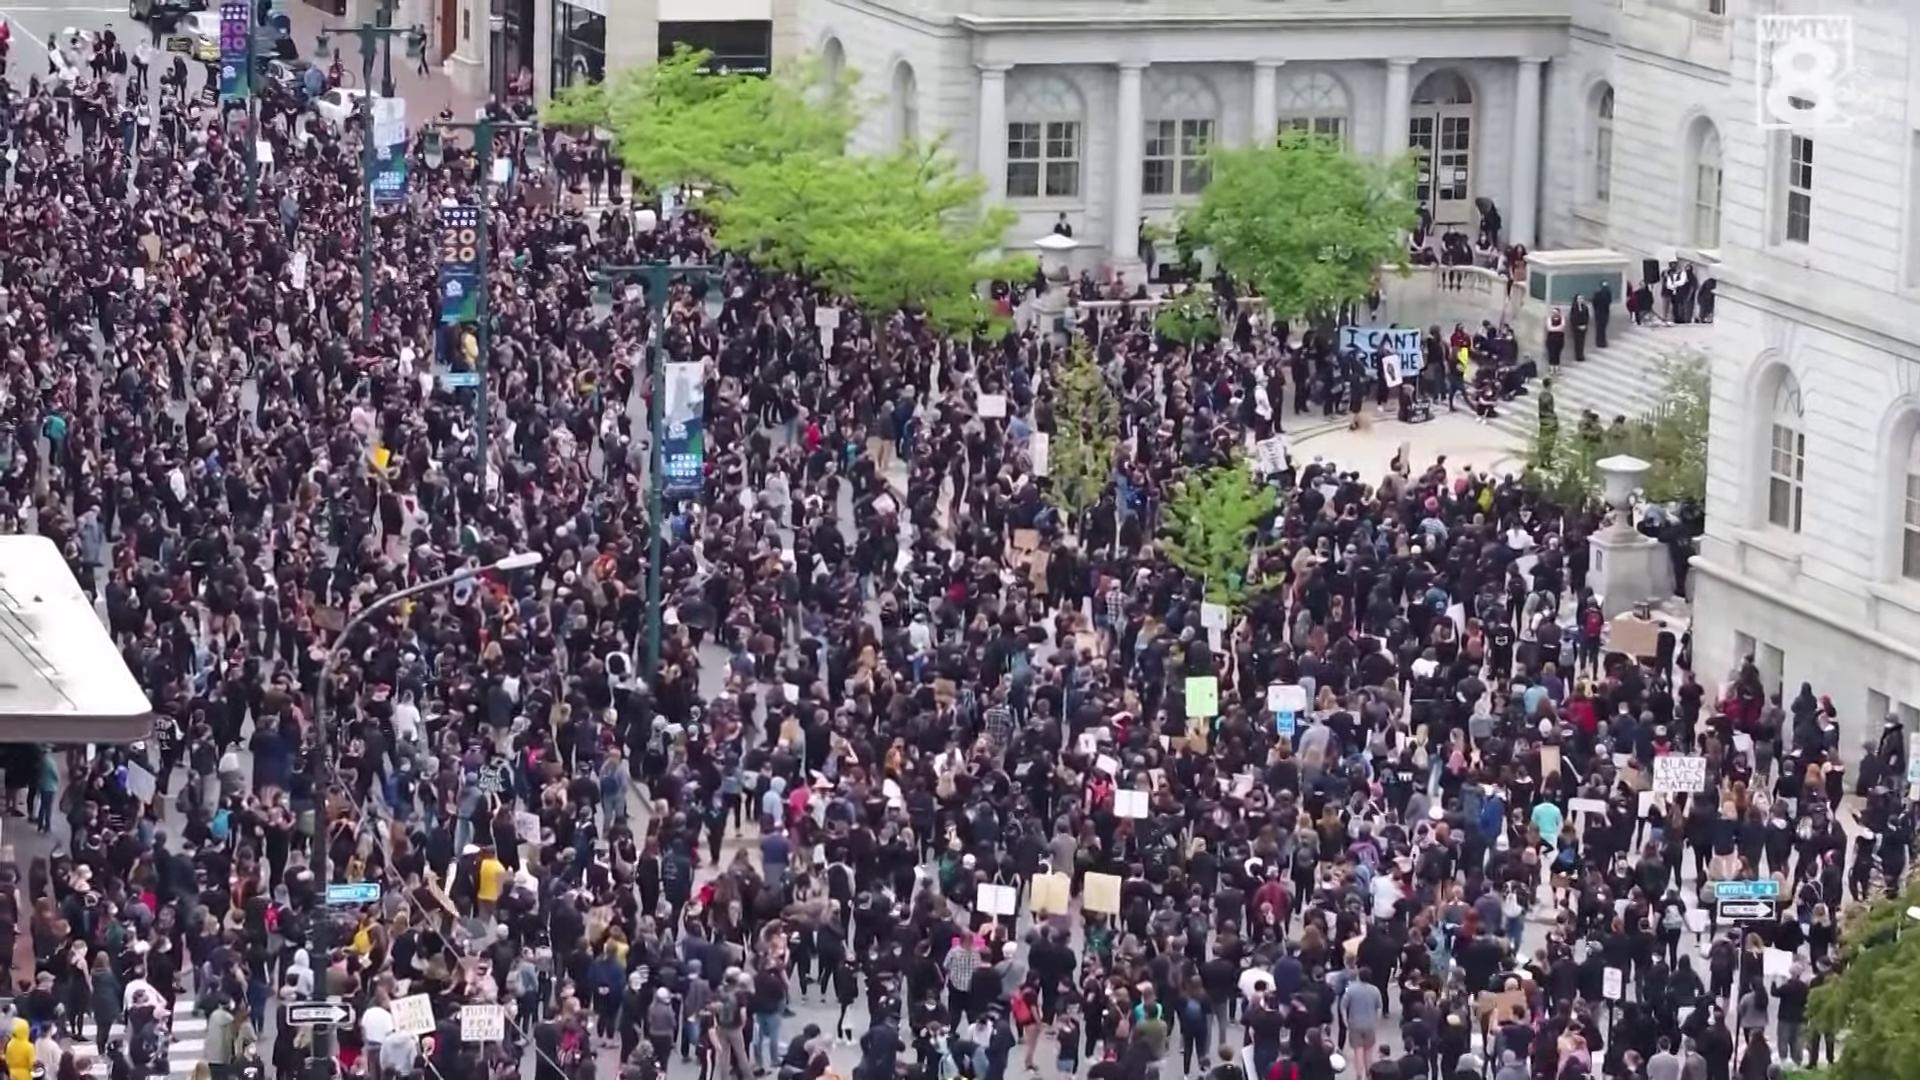
\includegraphics[height=8\baselineskip]{images/background/object_detection/5.jpg}} \quad \\
    \subcaptionbox{}{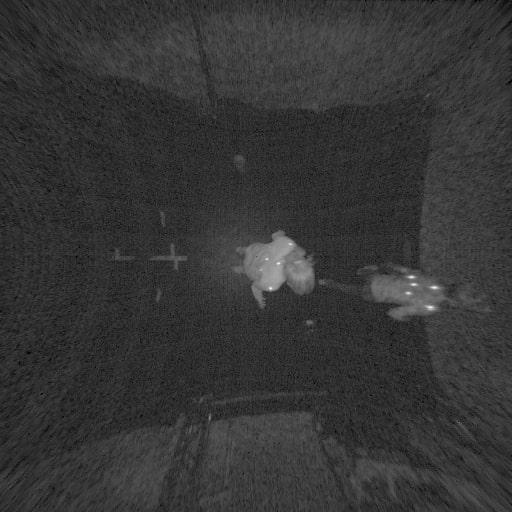
\includegraphics[height=8\baselineskip]{images/background/object_detection/ir.jpg}} \quad
    \subcaptionbox{}{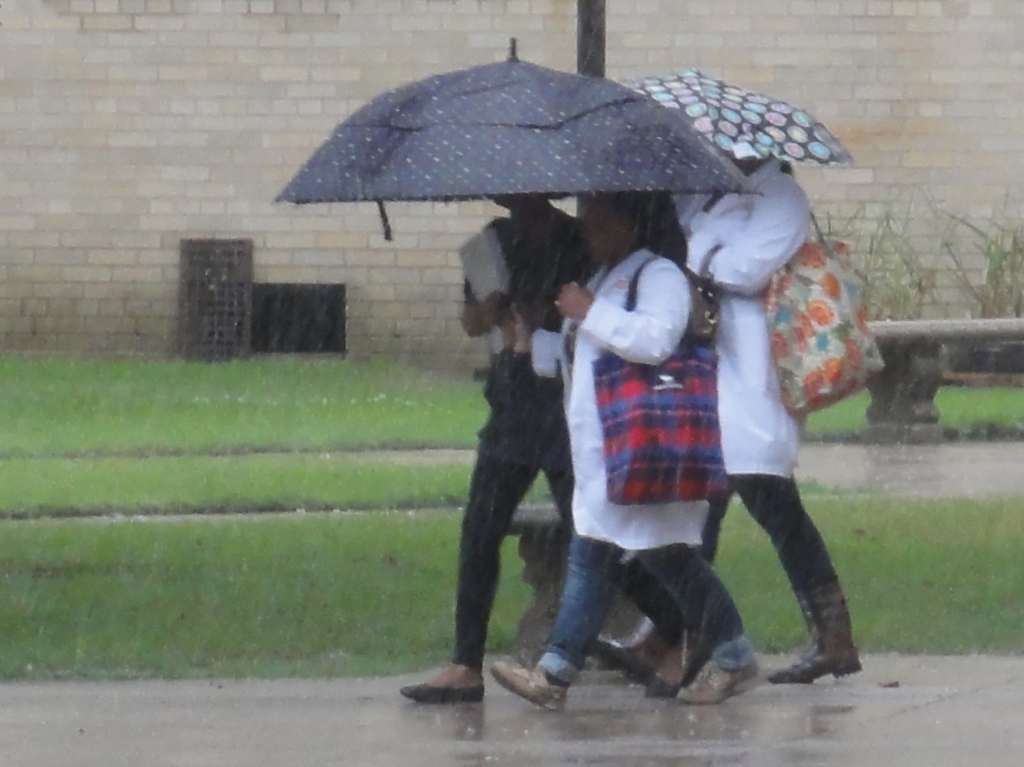
\includegraphics[height=8\baselineskip]{images/background/object_detection/occured.jpg}} \quad
    \caption{People can appear differently in various contexts \cite{kaggleCrowdDataset, viztaDataset, kaggleHumanDataset}}
   \label{fig:people}
\end{figure}

What makes a good object detection model generally depends on its intended use case. For example, a model deployed in a surveillance camera may require high speed and low computational cost, whereas in medical imaging, diagnostic precision is more critical. When comparing object detection algorithms, they are usually evaluated with classification metrics like average precision (AP), but also with other metrics such as inference speed and model size, using benchmark datasets like COCO (Common Objects in Context) \cite{lin2015microsoftcococommonobjects, algocomp, yolo11-docs, xin2024dartautomatedendtoendobject}. There can also be several case-dependent criteria for evaluation that need to be taken into account when training a model, such as scalability for retraining or the ability to handle certain edge cases. In the end, training a good object detection model requires handling several factors, which usually include selecting a suitable object detection model, providing a training dataset of appropriate size and quality, and applying preprocessing techniques.

Next, subsections \ref{sec:object_detection_methods} and \ref{sec:object_detection_evaluation_metrics} will discuss different object detection methods with a brief historical overview and introduce the most important object detection metrics used in this work. Later, chapter \ref{sec:workflow} will present a general perspective on object detection workflows.

\subsection{Object Detection Methods}
\label{sec:object_detection_methods}
Object detection techniques have improved a lot over the last decades. It could be said that the history of object detection can be roughly divided into two historical periods: the period of traditional object detection, which is the time before the year 2014, and the period of deep learning-based detection, which is after that \cite{object_detection_20years}. Correspondingly, object detection methods can be divided into traditional and deep learning-based approaches \cite{object_detection_review}. Next, traditional and deep learning-based\footnote{This section discusses different types of deep learning architectures and related terms, such as CNNs and transformers. These topics are introduced in more detail later in Section~\ref{sec:deep_learning}.} object detection methods are introduced in the context of these two historical periods.

Traditional object detection algorithms were mostly created on the basis of handcrafted features. Usually, the problem was the lack of advanced image representation and computational resources. Methods like the Viola-Jones detector (VJ detector) from 2001, Histogram of Oriented Gradients (HOG), and Deformable Part Models (DPM) were popular in traditional object detection. \cite{object_detection_review, object_detection_20years} Traditional object detection has three basic steps: informative region selection, feature extraction, and classification. As these steps included handcrafted features, generally traditional object detection models had difficulties with different domains and detections with complex backgrounds and diverse objects. \cite{SUN2024108458} These problems became easier to handle later with deep learning-based object detection models.

%Kirjoita jotain että teoria selitetään kappaleessa xxxx
The second turning point in object detection was initiated in 2012 when the deep learning model AlexNet \cite{alexnet} was introduced in the ImageNet Large Scale Visual Recognition Challenge (ILSVRC). AlexNet included, for example, convolutional neural network (CNN) architecture and the ReLU activation function. The achieved results got a lot of attention for using CNNs in object detection, and after 2014, when Regions with CNN features (RCNNs) were proposed by Girshick et al. \cite{RCNN}, object detection algorithms started to evolve faster than ever \cite{object_detection_20years}. After 2017, when Vaswani et al. \cite{vaswani2023attentionneed} introduced the transformer architecture, it became very popular in the field of natural language processing (NLP) and was applied very well also in other tasks like object detection. This becomes a point where modern deep learning-based object detection methods can be divided into two main categories: CNN-based and transformer-based object detection methods. \cite{SUN2024108458}

\begin{figure}
    \centering
    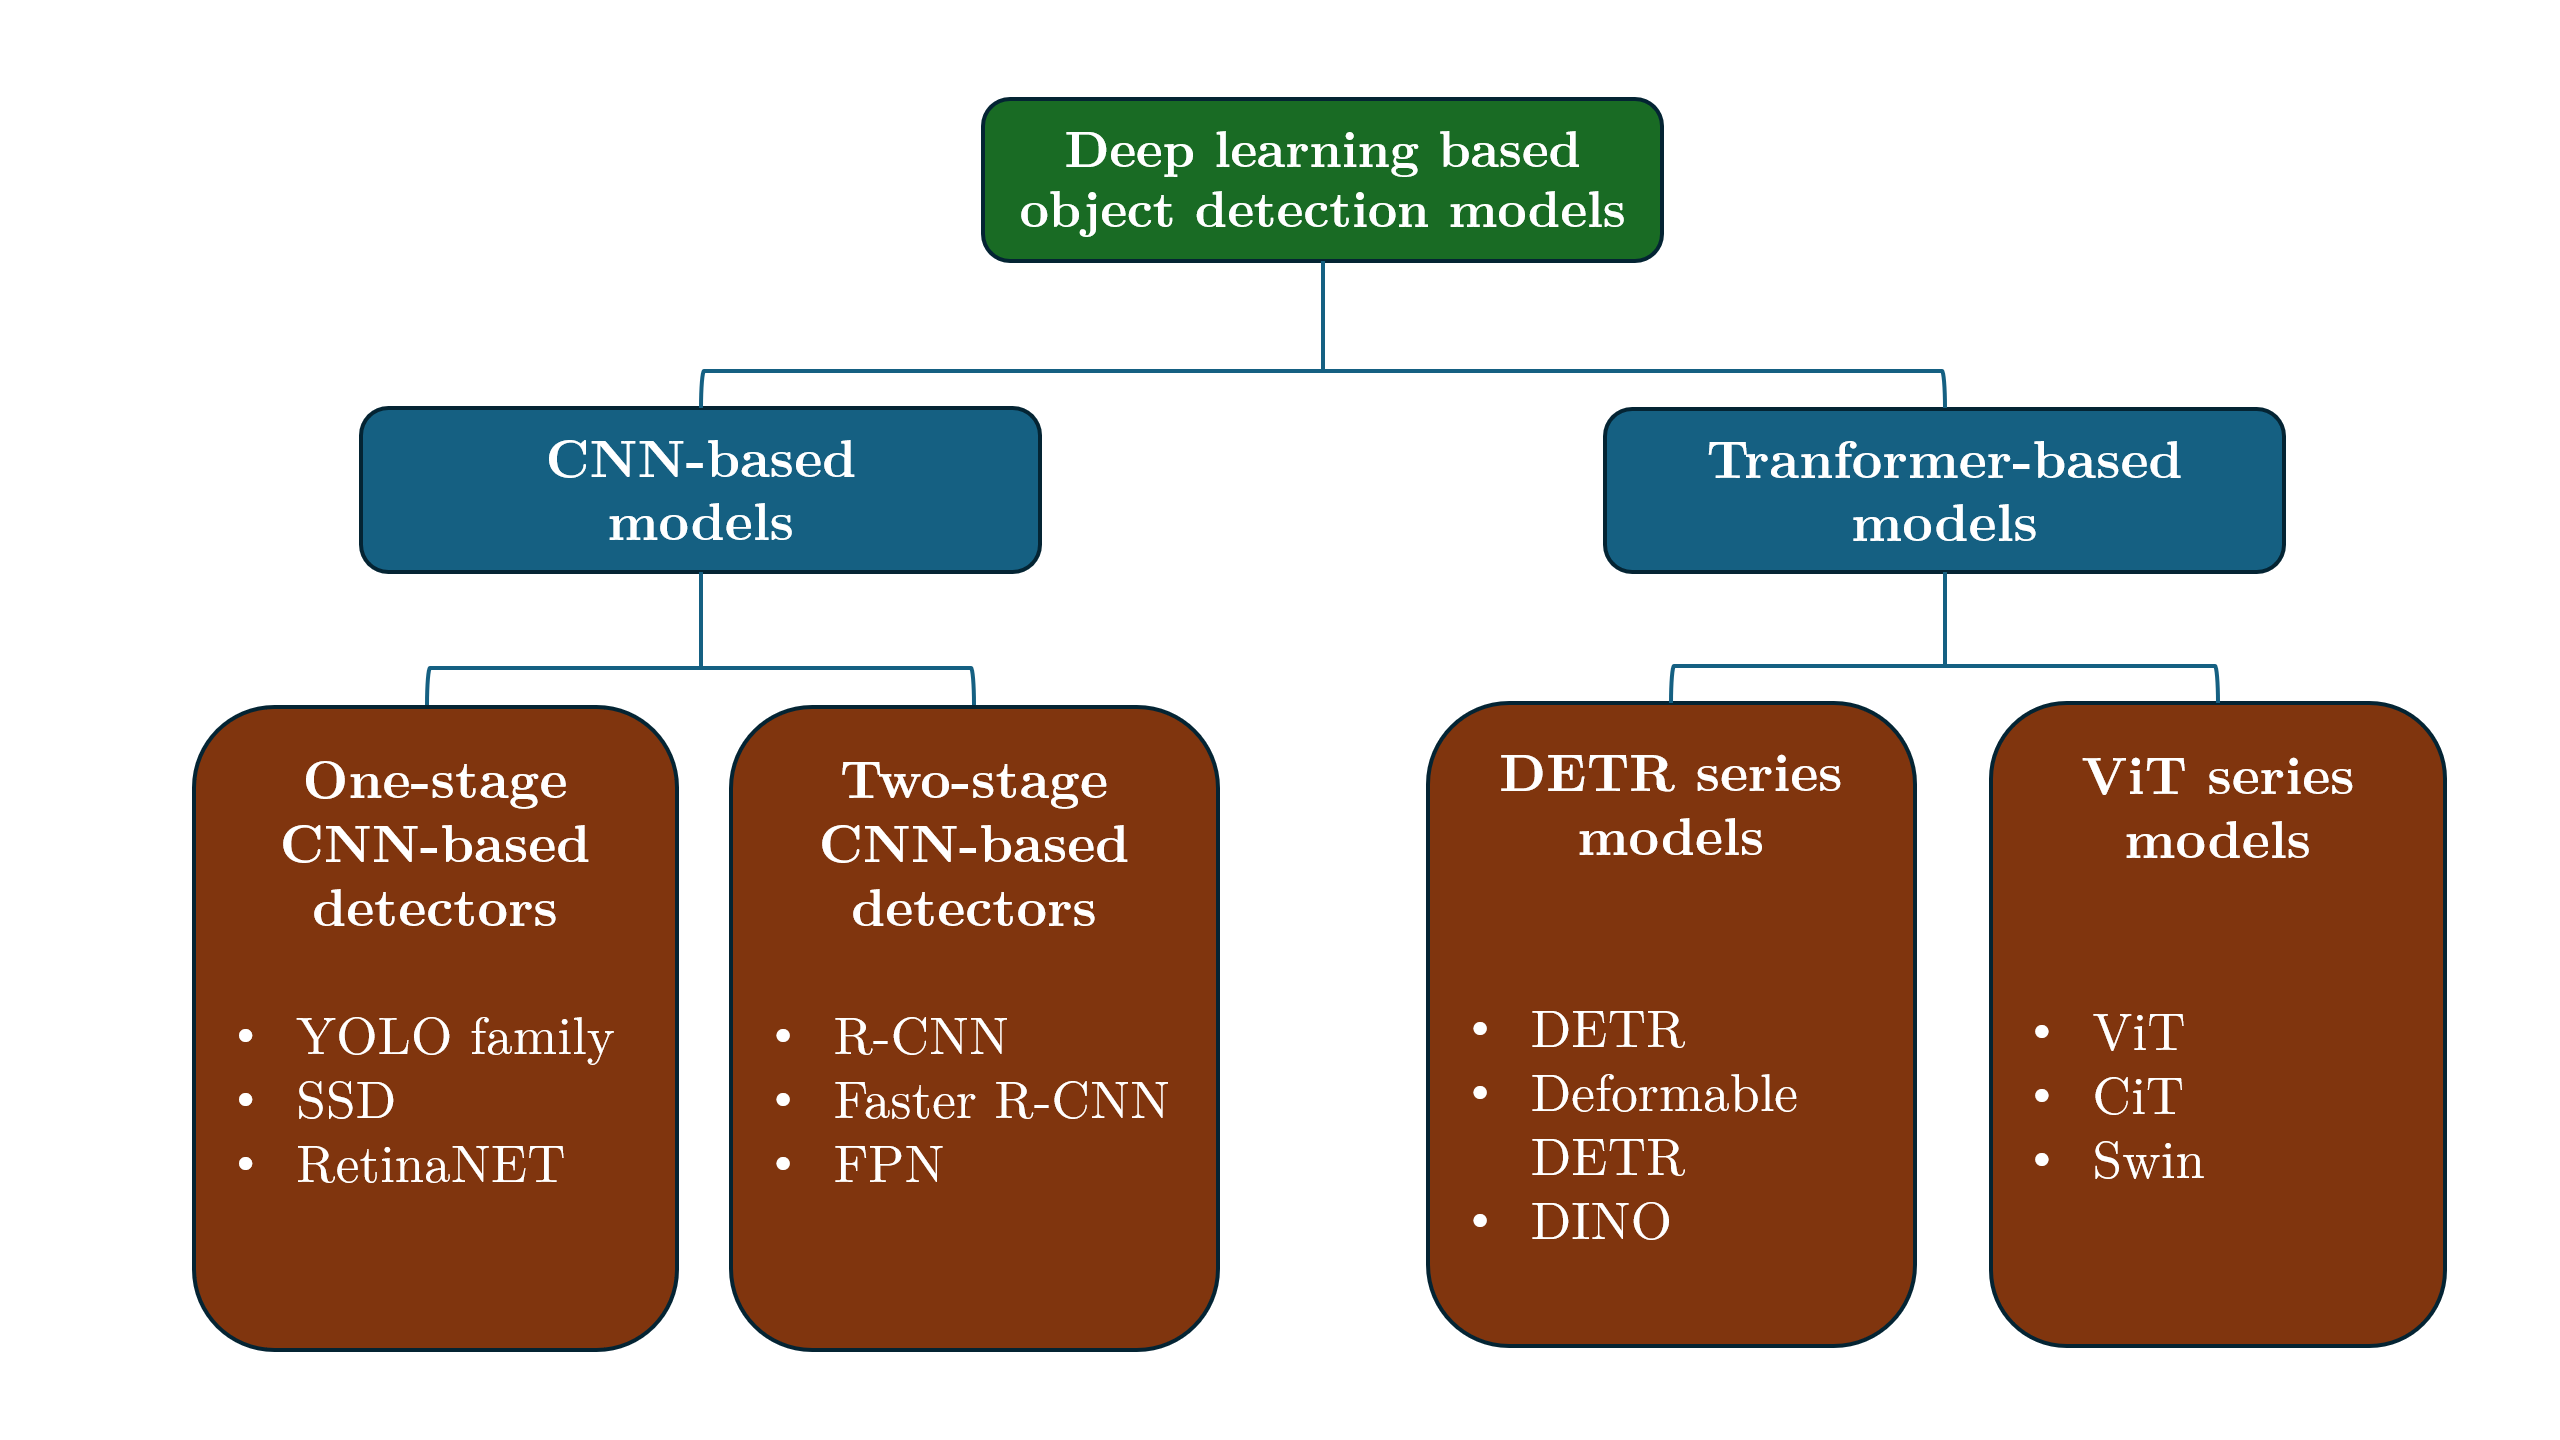
\includegraphics[width=1\textwidth]{images/background/history/models_new.png}
    \caption{Deep learning based object detection classification diagram}
   \label{fig:classdiagram}
\end{figure}

CNN-based deep learning object detection methods are usually divided into two main categories: one-stage detectors and two-stage detectors \cite{object_detection_review}. The most popular one-stage detectors are particularly the YOLO (You Only Look Once) family. For two-stage detectors, there are various popular options like R-CNN, Faster R-CNN, and feature pyramid network (FPN). These two methods differ from each other in how they detect objects from the data. One-stage detectors can classify and localize objects in one-step inference by extracting features with the CNN directly. Two-stage detectors first search for potential objects using region proposal algorithms like Selective Search or Region Proposal Networks (RPNs) and then classify and localize each proposed region by using CNN. \cite{SUN2024108458} Due to the complexity of two-stage detectors, compared to one-stage detectors they are usually more accurate, precise at localization, robust to occlusions, and better at handling complex scenes and small objects. However, two-stage detectors' inference speed is slower, they are computationally expensive, and complex to train \cite{Mukhopadhyay2024, onetwo}. These advantages and disadvantages suggest that one-stage detectors are better suited for real-time applications such as surveillance cameras and two-stage detectors may be more appropriate for accuracy-sensitive cases like medical image analysis. However, these differences are not so big nowadays as models are improving continuously. For example, \cite{SHARMA2024100648} reports that YOLOv8 achieved higher results than Faster RCNN in both accuracy and inference time.
 %Based on these advantages and disadvantages, the most popular application for one-stage detectors is real-time applications like surveillance cameras, and for two-stage detectors, medical image analysis.
%YOLO1-10 [https://arxiv.org/html/2408.09332v1]

Transformer-based object detection methods are quite new compared to CNN-based methods, as before 2020 there were no transformer-based object detection models until Carion et al. detection transformers (DETR) \cite{carion} and Dosovitskiy et al. Vision transformers \cite{dosovitskiy}. These methods can be divided into two categories: DETR series models and ViT series models. The idea of transformers lies in the self-attention mechanism, which makes the model able to pay more attention to the position of sequence features and the relationship between them. DETR models focus on end-to-end object detection by using a transformer encoder-decoder architecture, while ViT models are designed for general vision tasks like image classification by processing images as sequences of patches, and so ViT series models are usually used as backbones in object detection models. \cite{SUN2024108458} The performance of these models is sometimes said to be better than CNN-based models in larger datasets, but they are generally slower, larger, and more memory-intensive than traditional models \cite{Mukhopadhyay2024, battery, inproceedings}. Recently, there has been research that tries to improve the performance by combining CNN and transformer models like DEYOv2 \cite{DEYOv2}, but in this work it will be left out of discussion.


\subsection{Object Detection Evaluation Metrics}
\label{sec:object_detection_evaluation_metrics}
Object detection performance is mainly evaluated by localization and classification tasks. When comparing different object detection models, many other metrics related to model properties, like inference time, model size, and floating-point operations (FLOPs), can be included \cite{modelcomparison}. In this work, the focus is on detection rather than model computational performance; therefore, only the most common metrics used to evaluate the performance of localization and classification will be introduced, starting with localization.

A common way to measure localization performance is to evaluate the overlapped area between predicted and ground truth bounding boxes. This measure is called Intersection over Union (IoU), and it's defined as

\begin{equation}
    IoU = \frac{A_{Overlap}}{A_{Union}} \,.
\end{equation}

In the formula, $A_{Overlap}$ is the overlapping area between the detected bounding box and ground truth bounding box. $A_{Union}$ is the combined area of detected and ground truth bounding box. \cite{performancesurvey} The closer the IoU value is to 1, the better the localization is.

\begin{figure}
    \centering
    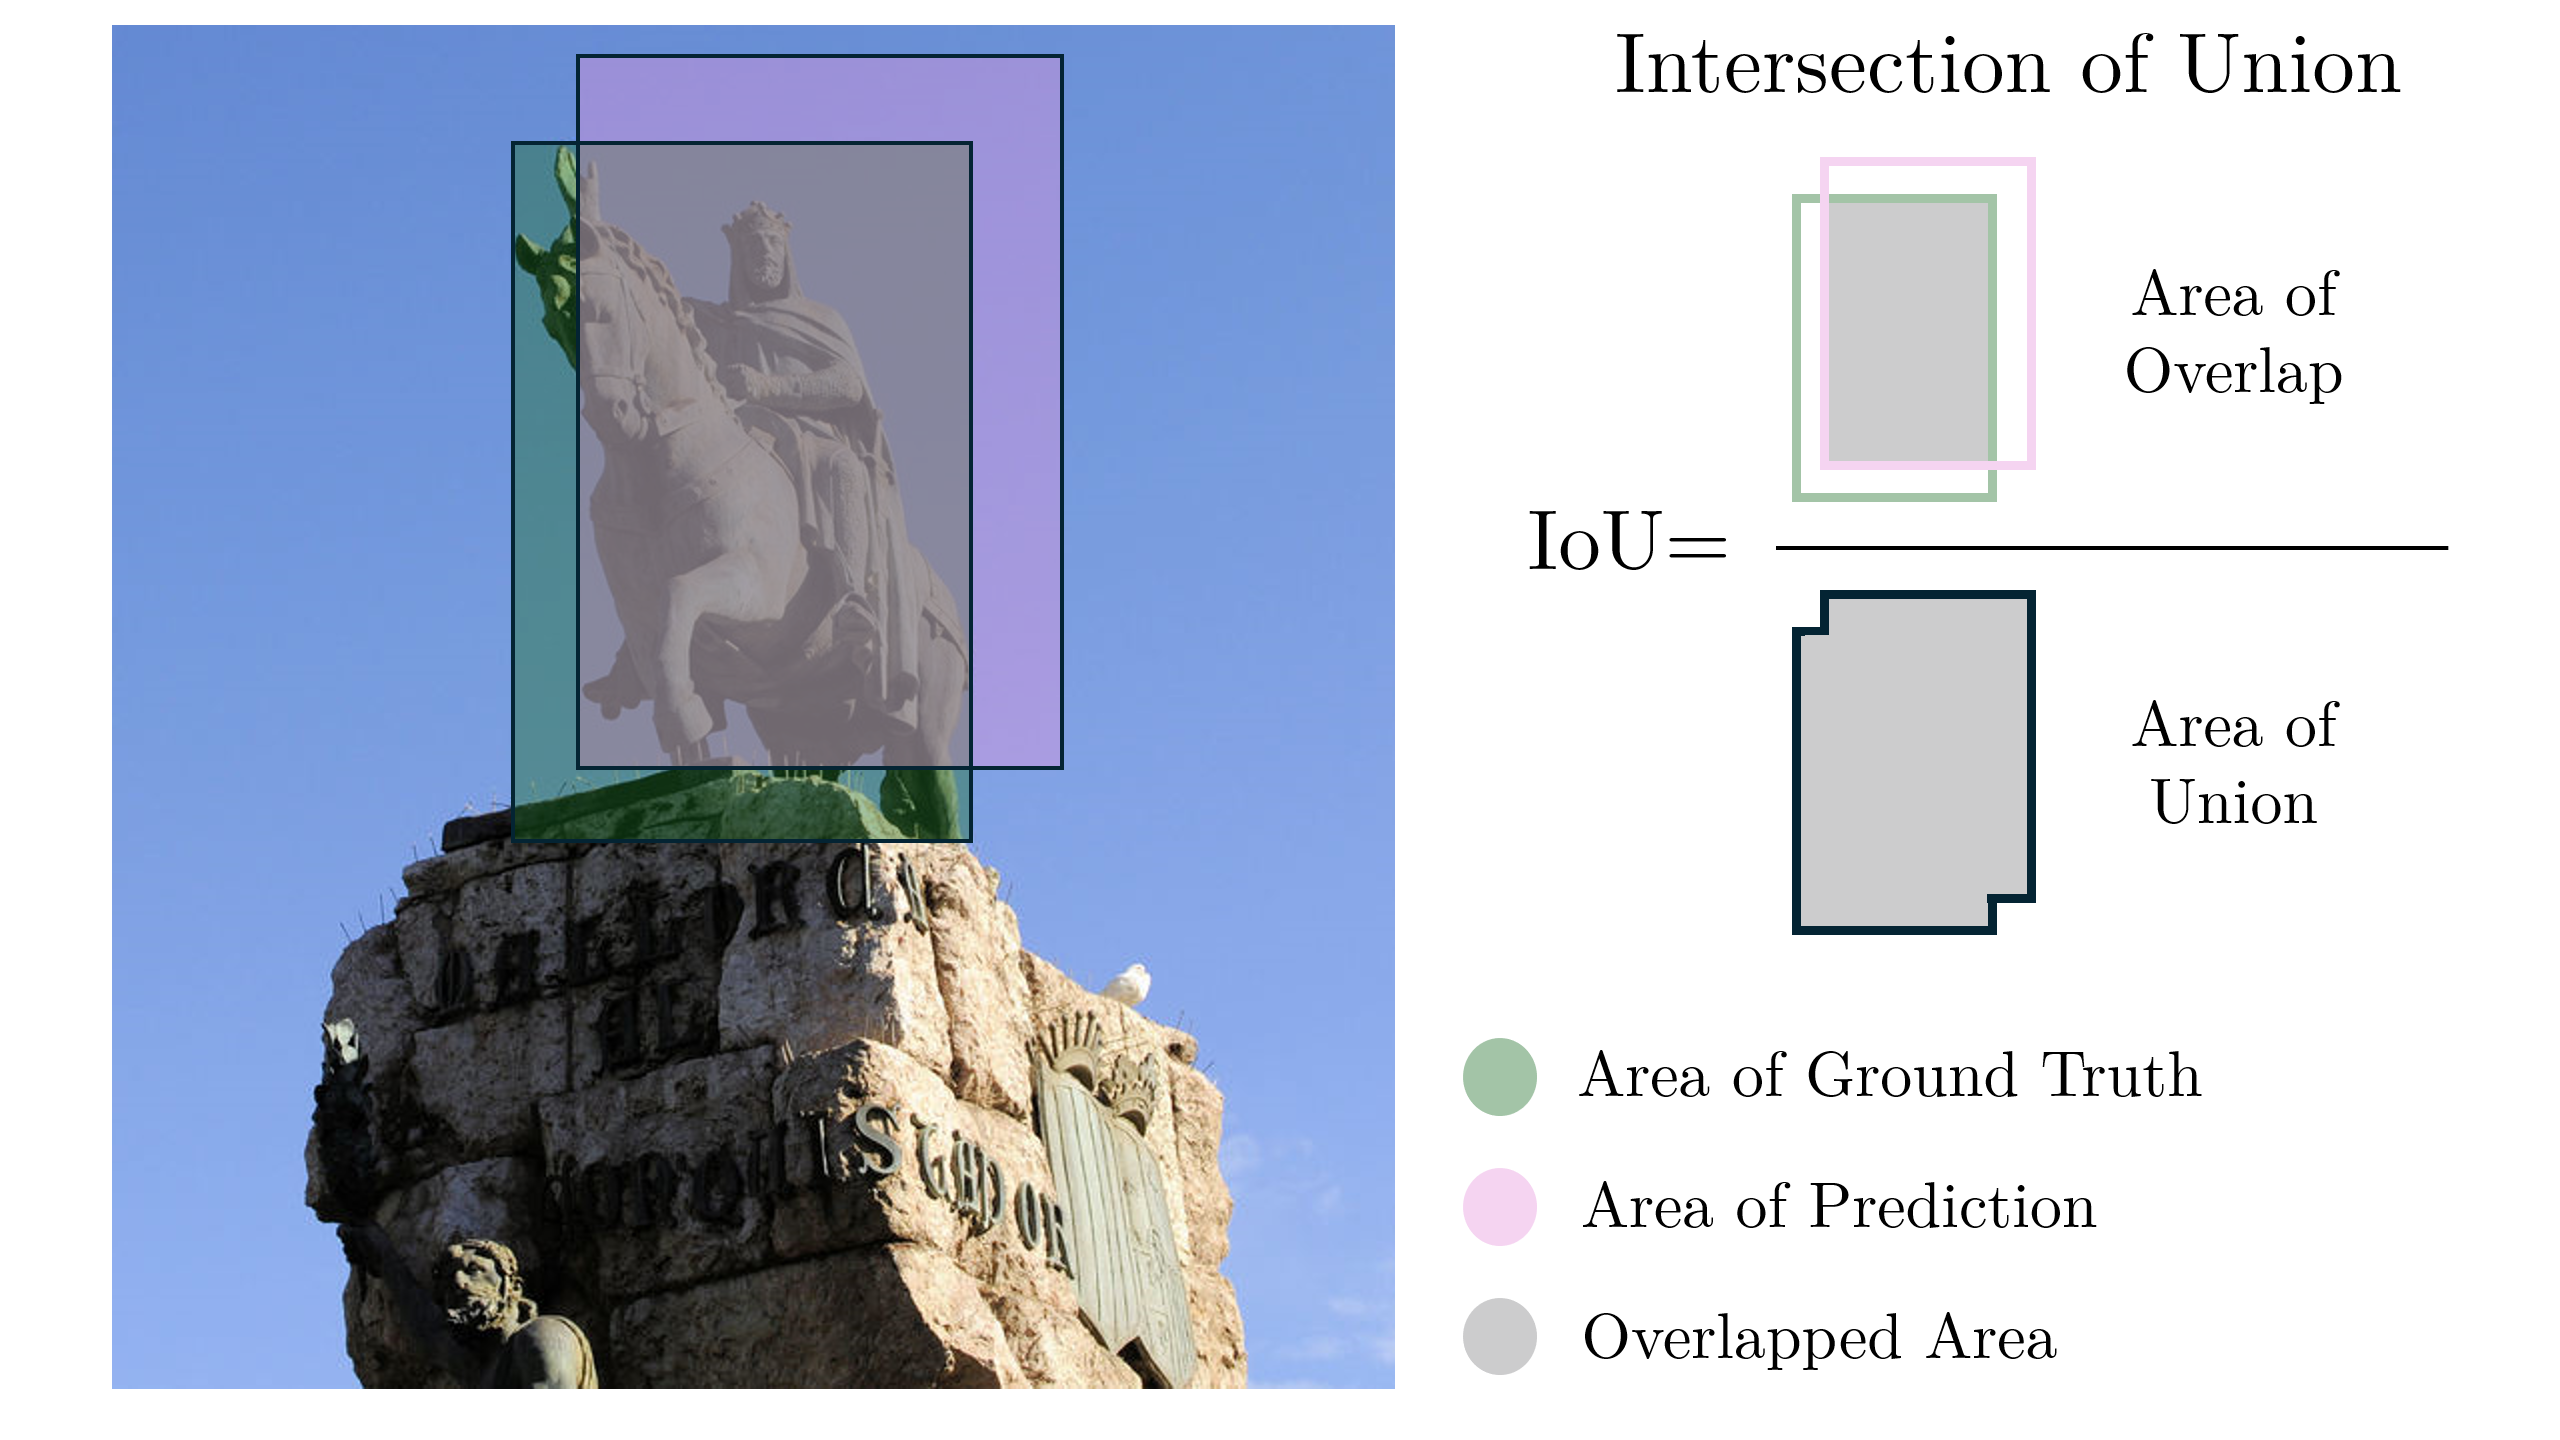
\includegraphics[width=1\textwidth]{images/background/metrics/iou_new.PNG}
    \caption{IoU is calculated as the area of overlap between the predicted and the ground truth bounding box divided by the area of union.}
   \label{fig:CNN_featurs}
\end{figure}

In practice, IoU is used to classify a detection as correct or incorrect with a given threshold. If IoU is greater or equal to the given threshold, it is classified as correct; otherwise, incorrect. \cite{performancesurvey}
IoU can also be used for removing duplicate bounding boxes in detection. Non-maximum suppression (NMS) is an algorithm used to eliminate overlapping bounding boxes and reduce duplicate detections. First, the algorithm selects the bounding box with the highest confidence score. Then IoU is calculated between this box and all other boxes with lower confidence. Any boxes with an IoU greater than a predefined threshold are discarded. This process is repeated: the next highest-confidence box among the remaining boxes is selected, and this process continues until only boxes with locally maximum confidence scores remain. \cite{NMS}
%The NMS algorithm is used in this work \url{https://docs.ultralytics.com/usage/cfg/}.

There are several different metrics to evaluate classification performance. These metrics are derived from the confusion matrix, which is a table that describes different outcomes of classification. In a binary classification task, the confusion matrix has four different outcomes: True positive (TP), True negative (TN), False positive (FP), and False negative (FN). \cite{Terven_2025} The confusion matrix for a binary classification task is defined as:

\begin{table}[!h]
    \centering
    \small % Reduce font size
    \begin{tabular}{c|p{4cm}|p{4cm}} % Adjust column widths
    & \textbf{Predicted Positive} & \textbf{Predicted Negative} \\
    \hline
    \textbf{Actual Positive} & 
    \begin{tabular}{@{}p{4cm}@{}}
        \textbf{True Positive (TP)} \\
        \small{\raggedright Object detected correctly}
    \end{tabular} & 
    \begin{tabular}{@{}p{4cm}@{}}
        \textbf{False Negative (FN)} \\
        \small{\raggedright Object not detected, but exists}
    \end{tabular} \\
    \hline
    \textbf{Actual Negative} & 
    \begin{tabular}{@{}p{4cm}@{}}
        \textbf{False Positive (FP)} \\
        \small{\raggedright Object detected, but does not exist}
    \end{tabular} & 
    \begin{tabular}{@{}p{4cm}@{}}
        \textbf{True Negative (TN)} \\
        \small{\raggedright Object not detected, and does not exist}
    \end{tabular} \\
    \end{tabular}
\end{table}

In this matrix, TP and TN represent correct predictions and likewise FP and FN represent incorrect predictions. It is good to note that TN is not generally used in object detection, because all images can have infinite number of bounding boxes that should not be detected \cite{performancesurvey}. Therefore TP, FP and FN are used to derive classification metrics precision, recall, average precision and F1-score \cite{Terven_2025}.
\newpage
Precision is the ratio of correctly detected positive cases to all made detections. It is defined as:

\begin{equation}
    Precision = \frac{TP}{TP + FP} \,.
\end{equation}

A low precision value indicates a high number of falsely detected objects in predicted data. Because of that, precision is an important metric, especially when false alarms are costly. However, since precision does not take into account missed detections, recall is also needed. \cite{Terven_2025}

Recall is the ratio of correctly detected positive cases to all positive ground truth cases, and it measures the model's ability to detect relevant instances. Recall is defined as:

\begin{equation}
    Recall = \frac{TP}{TP + FN}
\end{equation}

A low recall value indicates there is a high number of cases where objects are not detected even though they exist. \cite{Terven_2025}

Between precision and recall there is a trade-off: If precision increases, recall tends to decrease and vice versa \cite{Terven_2025}. This trade-off is generally influenced by the confidence score threshold: A higher confidence score threshold means more predictions are discarded due to a strict threshold and so there are more FN cases, meaning higher precision. A lower confidence score threshold means even uncertain predictions are accepted, which leads to greater FP cases and recall. This trade-off can be illustrated in a precision-recall curve (see Figure~\ref{fig:PR-curve}), where values are plotted at confidence score threshold values \cite{Terven_2025}.

\begin{figure}[H]
    \centering
    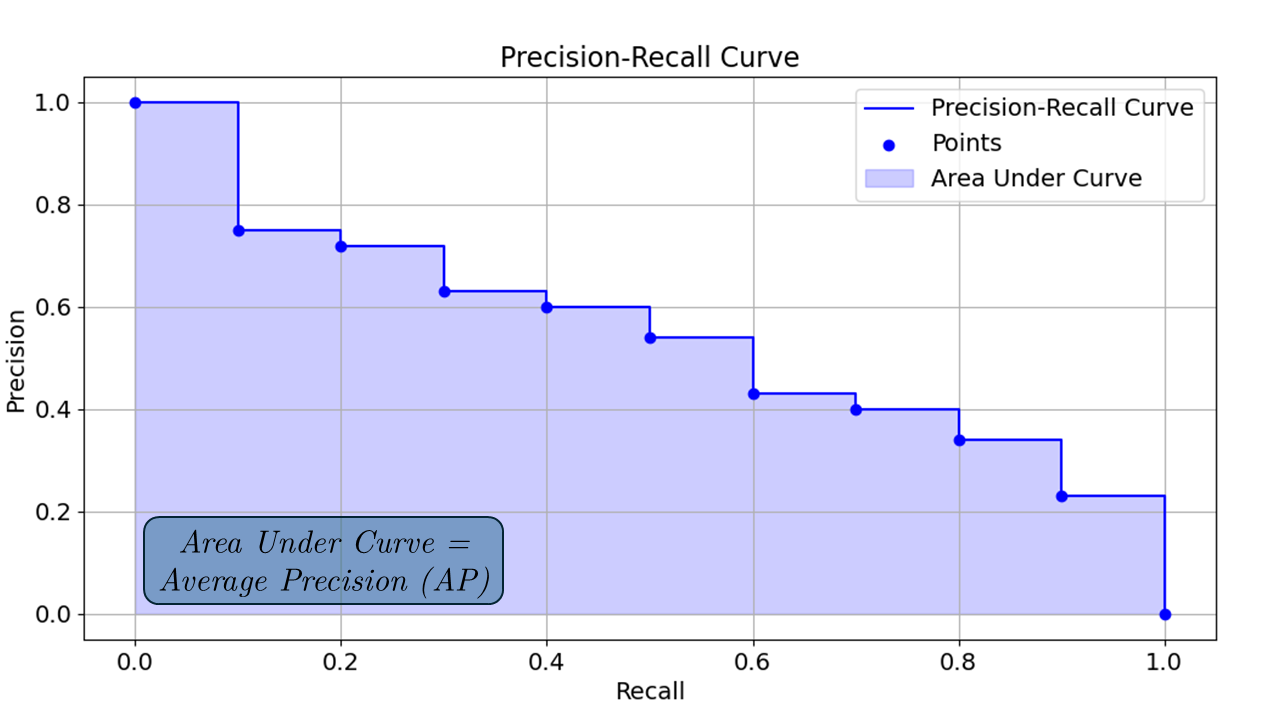
\includegraphics[width=0.93\textwidth]{images/background/metrics/pr.png}
    \caption{Example of a precision-recall curve using the 11-point interpolation approach.}
   \label{fig:PR-curve}
\end{figure}

In practice, models are often compared based on how well they maintain high recall before precision starts to drop fast. To represent this overall performance as a single numeric value, the information of the precision-recall curve is expressed as Average Precision (AP). Average Precision and its aggregate form, mean Average Precision (mAP), are very popular metrics to evaluate object detection models. AP is defined as the area under the precision-recall curve and can be expressed as:
\begin{equation}
    AP_{\tau} = \int_{0}^{1} p(r) dr \,,
\end{equation}
where $AP_{\tau}$ is AP at IOU threshold $\tau$ and $p(r)$ is the precision at recall $r$. \cite{Terven_2025} Mean Average Precision is the mean of the AP values of all object classes. mAP is defined as
\begin{equation}
    mAP = \frac{1}{n} \sum_{i=1}^{n} AP_i
\end{equation}
where $n$ is the number of classes and $AP_i$ is the AP of class $i$. \cite{performancesurvey} If there is only one class, mAP is equal to AP. It is important to note that there are different ways to calculate AP. For example, two widely used evaluation standards, Microsoft COCO and Pascal VOC, compute AP differently \cite{Terven_2025}. In this work, the Open-Source Visual Interface for Object Detection Metrics \cite{electronics10030279} is used to calculate AP using Pascal VOC AP computation. Often in literature, there are notations AP@0.50 or AP@[.50:.05:.95], which means that AP is calculated using different IoU thresholds. AP@50 refers to AP calculated using IoU threshold 0.5 and AP@[.50:.05:.95] means the average of AP values calculated using IoU thresholds from 0.5 to 0.95 with step size 0.05. \cite{Terven_2025}

As AP summarizes performance across all confidence score thresholds, it is usually necessary in practice to find a single confidence score threshold that gives the best balance between precision and recall. For this, the F1-score is used. F1-score is the harmonic mean of precision and recall:
\begin{equation}
    F1 = \frac{2}{\frac{1}{Precision} + \frac{1}{Recall}} = 2 \cdot \frac{Precision \cdot Recall}{Precision + Recall} \,.
    \label{eq:f1}
\end{equation}
One feature of the harmonic mean is that it penalizes large differences between precision and recall, so a high F1-score value indicates a good balance between those two metrics. \cite{Terven_2025}

In this work, AP is used as the main evaluation metric to measure overall performance for trained object detection models, while F1-score is used to find the optimal confidence score threshold for the models.


\section{Deep Learning Architectures}
\label{sec:deep_learning}

%LIST TASKS
Deep learning is a subset of machine learning that utilizes neural networks to solve complex tasks like object detection, image generation and natural language processing \cite{MLDL}. This section will, after a short refresher about neural networks, introduce the main information about convolutional neural networks (CNNs), U-Net, and transformers as they are related to object detection and text-to-image generation models used in this work.

\begin{figure}[!h]
    \centering
    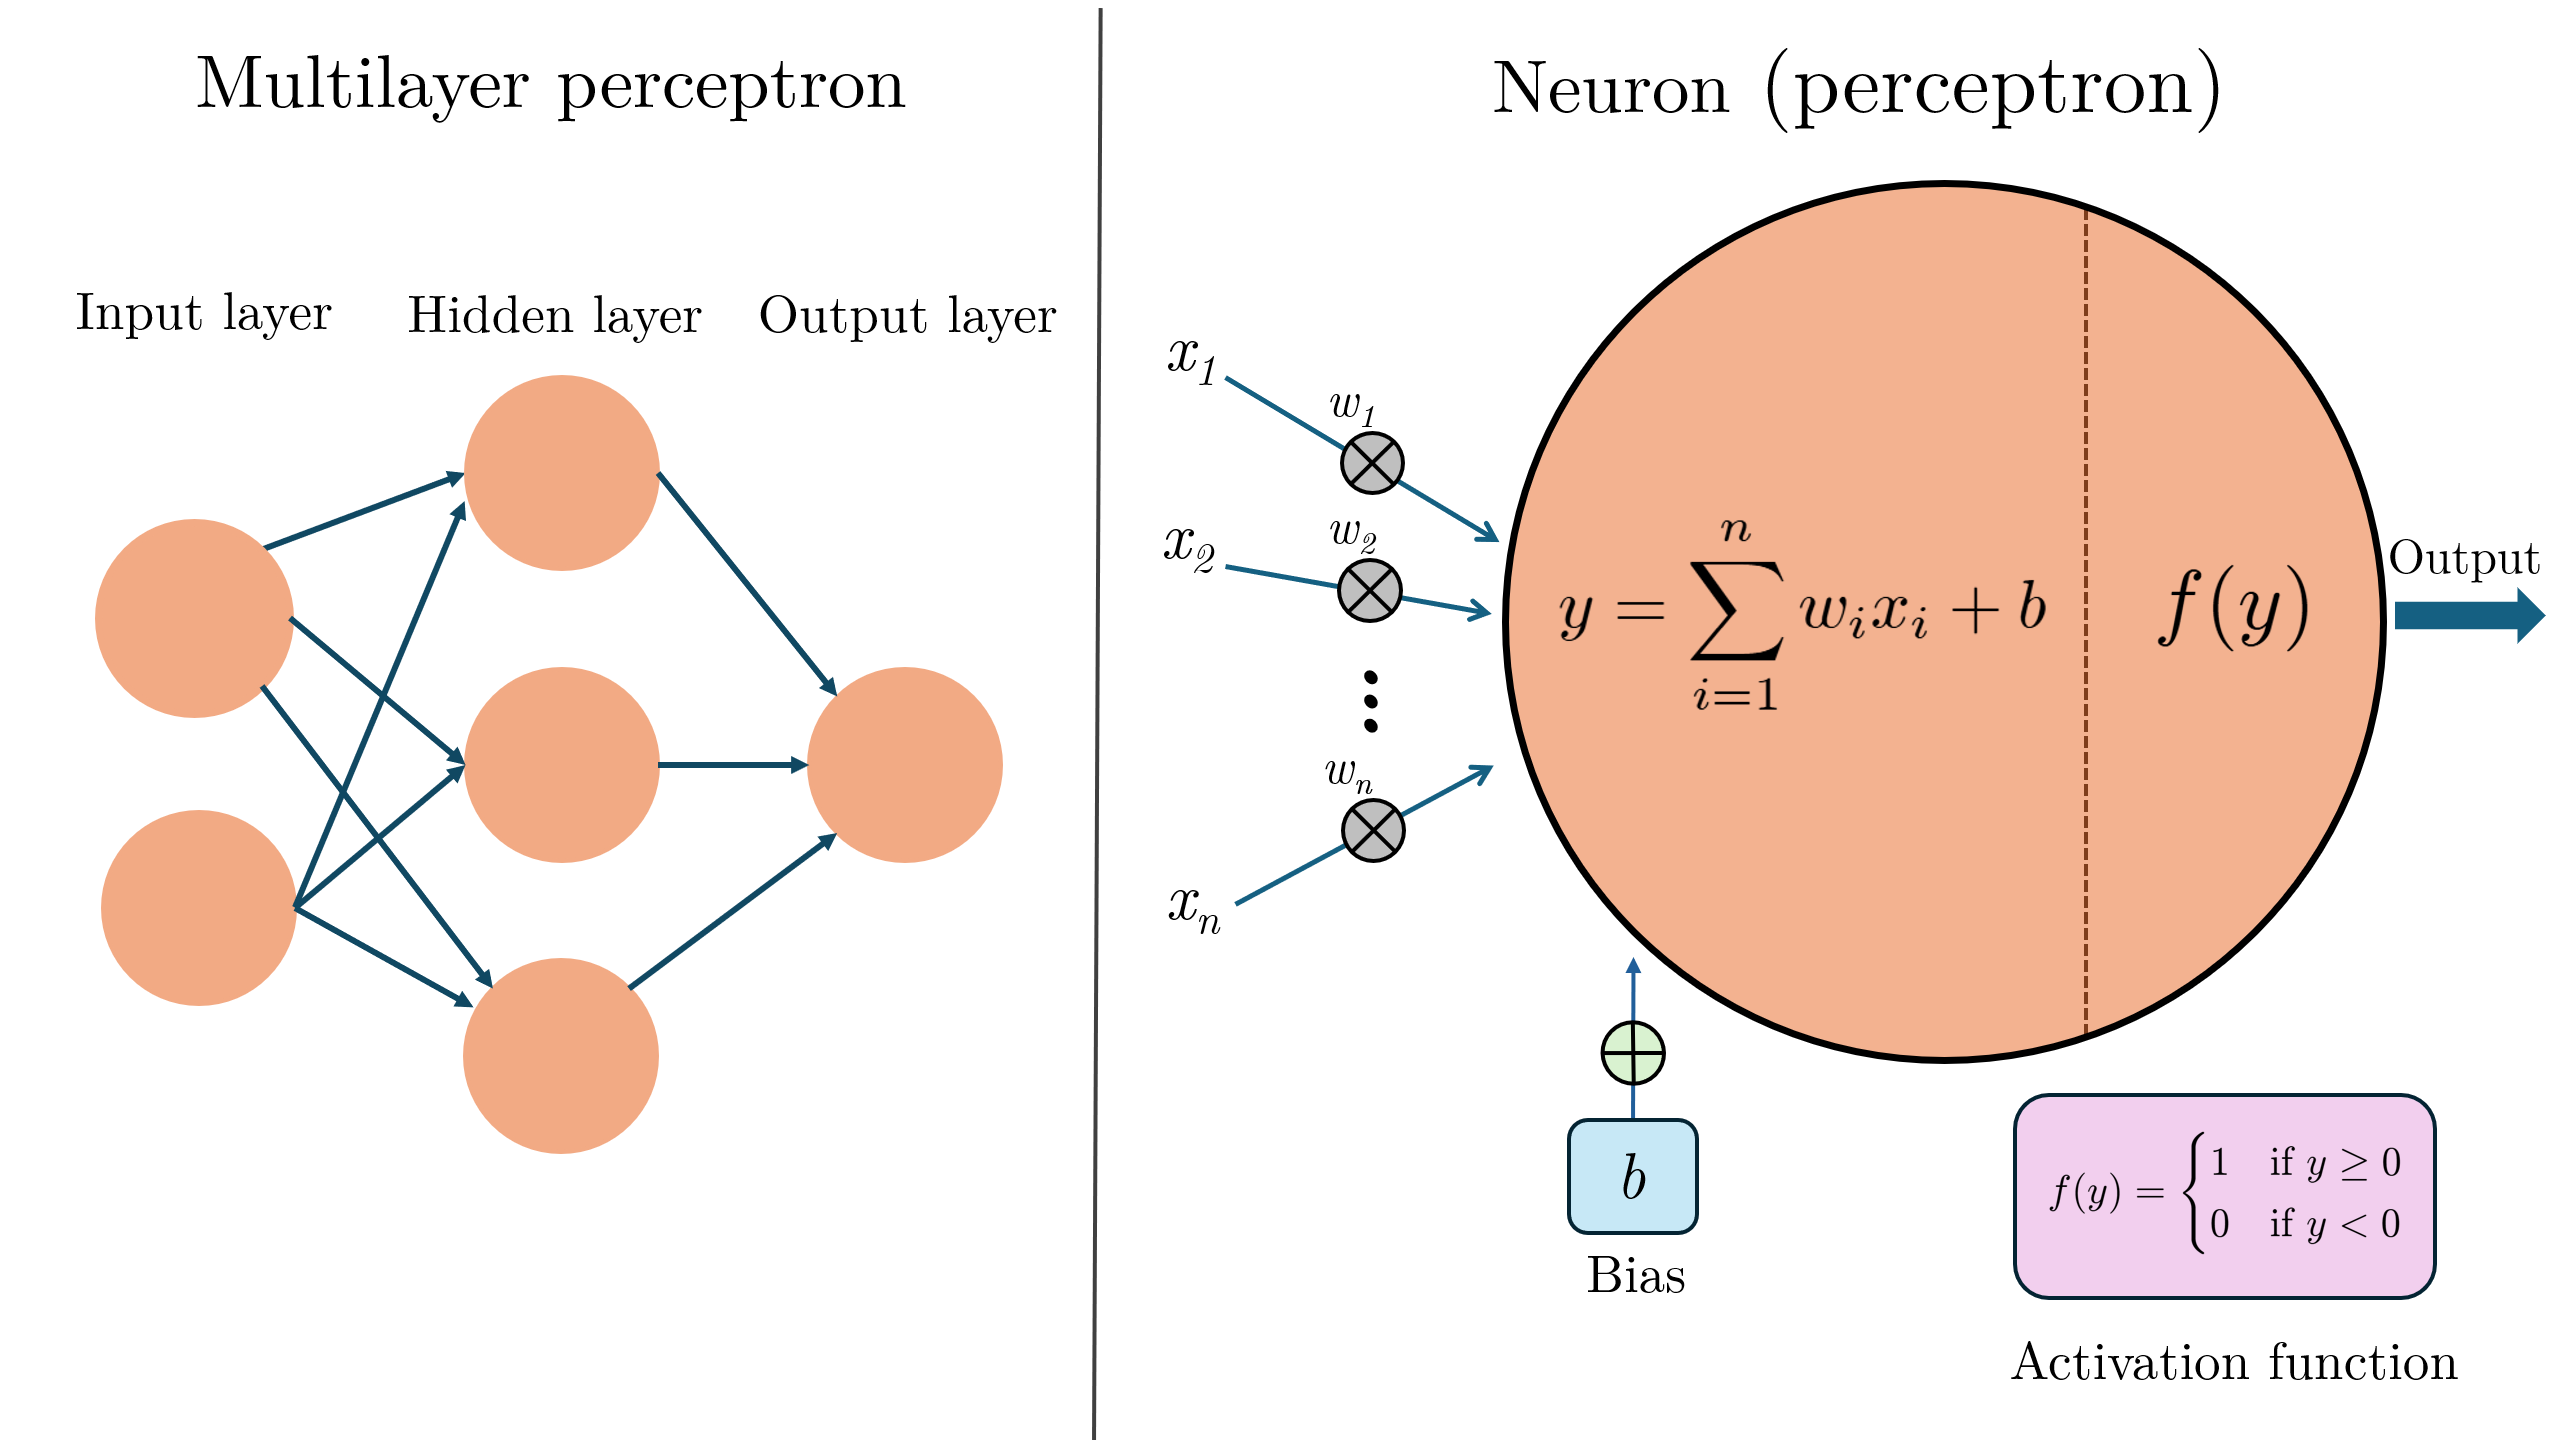
\includegraphics[width=1\textwidth]{images/background/CNN/perceptron_new.png}
    \caption{ Example of a simple multilayer perceptron and a neuron. The activation function is chosen to be the Heaviside step function in this example.}
   \label{fig:NN}
\end{figure}

Neural networks are collections of neurons, or computing units, that are connected to each other \cite{calin_deep_2020}. They are designed to be universal predictors\footnote{More information about the universal approximation theorem \cite{valle2024universalapproximationtheoremvector, lu2017expressivepowerneuralnetworks}.} that can be trained to learn complex relationships between input and output \cite{calin_deep_2020, gonzales}. While a single neuron, also called a perceptron, can mainly be used for binary classification, learning more complicated features requires several layers of neurons. A multilayer perceptron (MLP) is a type of neural network that consists of an input layer, an output layer, and possibly one or multiple hidden layers. In the MLP, each neuron in a layer is connected to all neurons in the next layer, creating a fully connected neural network. The input layer simply receives and passes forward the input data. In the hidden layers, all incoming input data to a neuron are multiplied by the weights assigned to those inputs, summed together, and then a single bias is added (compare to the equation of a line $y=ax+b$). The result of the summation is then passed through a mathematical function called an activation function, which gives an output based on the function used. Nowadays, activation functions are usually monotone increasing functions in practice, such as the logistic function, hyperbolic tangent function, or ReLU, which serve modern neural network architectures better. At the end of the network is the output layer, which is similar to a hidden layer but gives the final output and may use a different activation function compared to the hidden layers. \cite{calin_deep_2020, herberg2023lecturenotesneuralnetwork}

%The activation function used in the figure \ref{fig:NN}, the Heaviside funcion, which closely resembles orginal idea that a biological neuron fires only if the input exceeds a certain threshold.

%LOSS ENNEN MÄÄRITELMÄÄ
The goal of the neural network is to learn relationships between input and output, which can be achieved by learning the weights and biases that minimize the loss function. The loss function, also known as the cost or error function, measures the error between the predicted output and the ground truth output. During the training process, the weights and biases are usually adjusted using backpropagation and the gradient descent algorithm. The backpropagation algorithm computes gradients of the loss with respect to the weights and biases. The gradient descent optimization algorithm, or its popular variant stochastic gradient descent, is used to update the weights and biases in the direction that minimizes the loss function using gradients calculated from backpropagation. This iterative process is repeated at each step, with the step size determined by the learning rate, until the stopping criteria are met. \cite{calin_deep_2020,herberg2023lecturenotesneuralnetwork}

\subsection{Convolutional Neural Networks} 
\label{sec:CNN}
Convolutional neural networks (CNNs) are deep learning architectures that are commonly used for different computer vision problems, including object detection, image segmentation, and image classification \cite{10466766}. A CNN is a type of neural network that uses convolution kernels for feature extraction. A typical CNN architecture consists of convolutional layers, pooling layers, and fully connected layers, as seen in Figure~\ref{fig:CNN} \cite{CNNanalysis}. Convolutional and pooling layers perform feature extraction to learn relevant features for the fully connected layers, which map those features into the final output such as probabilities in classification tasks \cite{CNNradiology}.

\begin{figure}[!h]
    \centering
    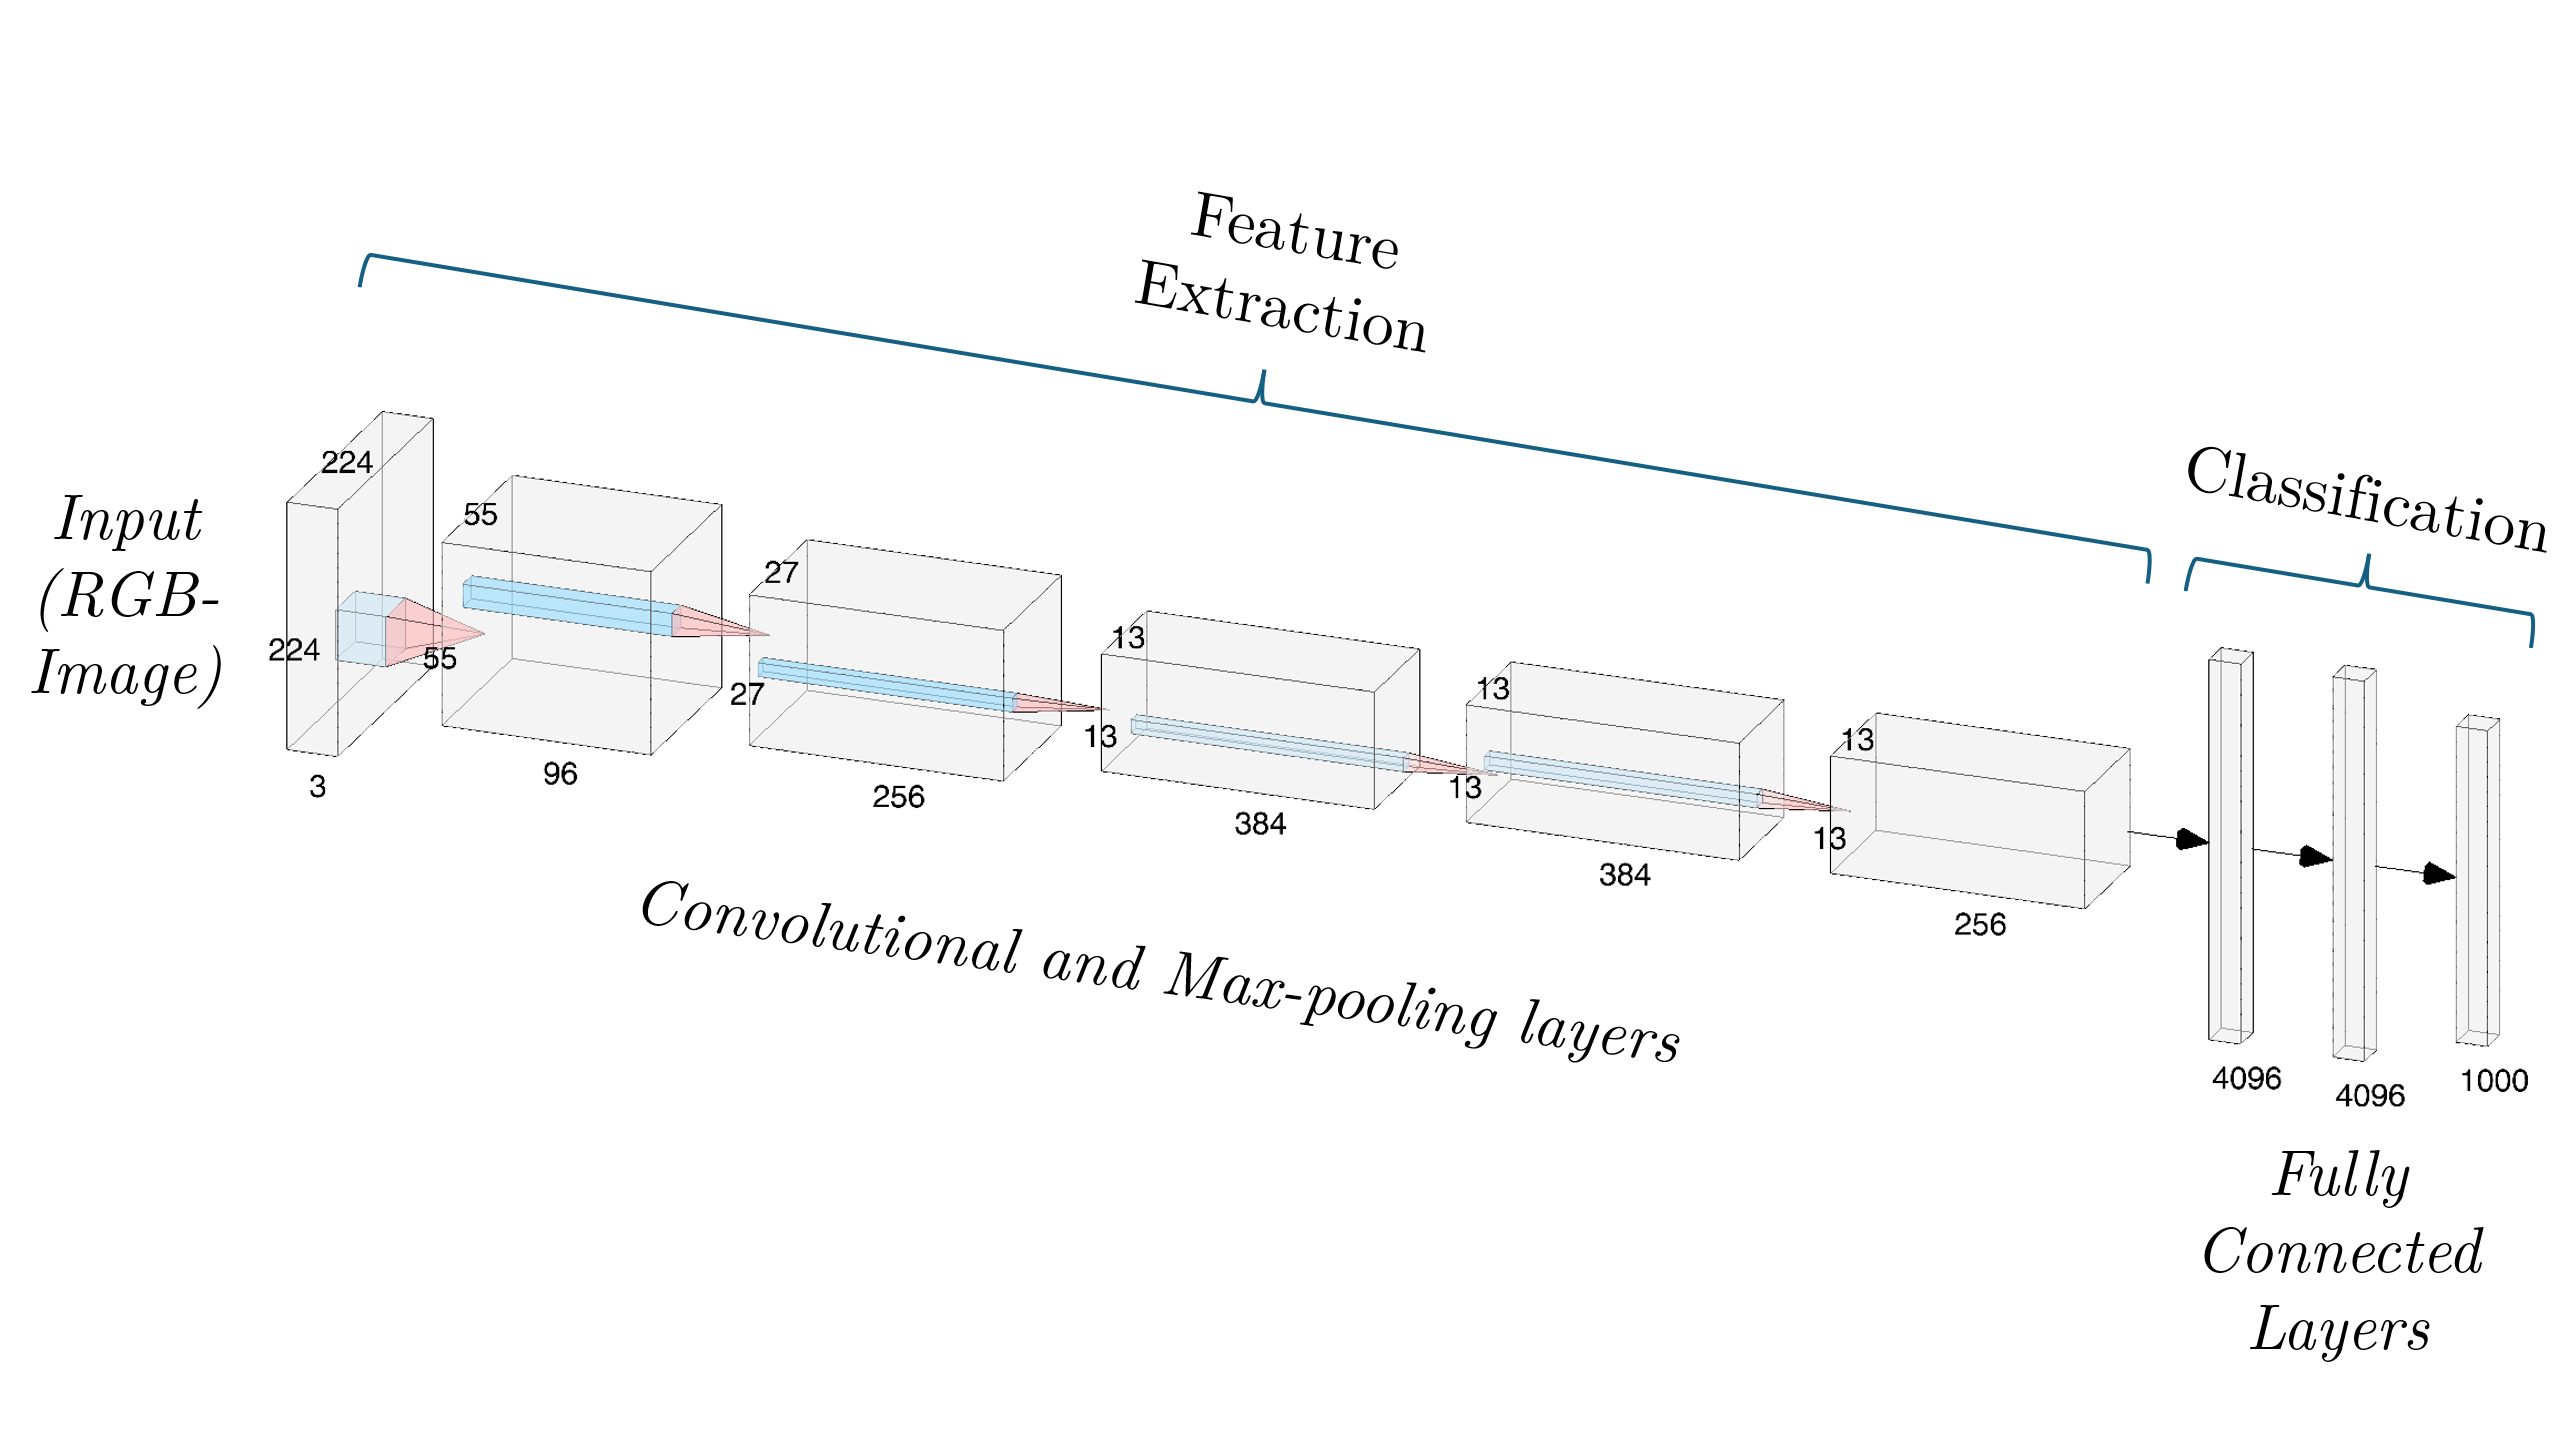
\includegraphics[width=1\textwidth]{images/background/CNN/CNN.png}
    \caption{Example of a CNN architecture.}
   \label{fig:CNN}
\end{figure}

In a convolutional layer, features are extracted from the input image using convolution kernels. Kernels are small weighted filters that are slid over the input image, computing at each step a convolution: a dot product between the kernel and an image patch of the same size. \cite{computation11030052} This produces a new image called a feature map. Each feature map highlights different features, such as edges, corners, or textures, depending on the kernel's weights. As the kernel weights do not change while sliding over the image (also known as weight sharing), it allows the detection of the same features across the image while reducing the number of parameters, which is a key feature of the convolution operation. In a convolutional layer, there are multiple different kernels that extract different features, as their weights are different. \cite{CNNradiology} For example, in Figure~\ref{fig:CNN}, the first convolution layer of the CNN has 96 kernels. Kernels are learnable parameters that are adjusted during the training process so they can extract meaningful features from the input image \cite{computation11030052}. Other important parts of the convolutional layer are zero padding and the activation function. Zero padding is a technique where the input image is padded with zeros on each side so the feature map will not get smaller with each convolution operation. At the end of the convolutional layer, the rectified linear unit (ReLU) activation function is usually used. ReLU is a nonlinear activation function that returns 0 if the input is negative and otherwise returns the input value. \cite{CNNradiology} The idea of using ReLU is to avoid vanishing gradients and to keep the activation function computationally cheap \cite{herberg2023lecturenotesneuralnetwork}.

In pooling layers, feature maps are downsampled. This reduces the number of subsequent learnable parameters and increases the field of view of the feature maps, which enables the next convolutional layers to capture more complex features while enhancing earlier features. Downsampling is usually done by max pooling, where a small sliding window returns only the maximum value from a feature map patch, or by average pooling, where it returns the average value from a feature map patch. \cite{CNNradiology}

At the end of the CNN, after the features are extracted, feature maps are flattened and passed to fully connected layers, also called dense layers. This is similar to the MLP, where each neuron in the layer is connected to all neurons in the next layer, also having learnable parameters like weights. Fully connected layers are used to classify the features extracted from the image. In image classification, the output layer gives a vector of probabilities for each possible class. To scale probabilities between 0 and 1 while ensuring their sum equals 1, the softmax activation function is used in the output layer. \cite{CNNradiology}
Comparing a generic CNN architecture to the first YOLO object detection model, which is also a CNN, the output layer predicts four coordinates of the bounding box, a confidence score, and the class. In YOLO, the output layer is a 7x7x30 tensor, where 7x7 comes from the original image being divided into 7x7 grid cells. Each grid cell predicts 30 values, which are probabilities for 20 detectable objects and 2 bounding boxes, each having four coordinates and a confidence score. \cite{redmon2016lookonceunifiedrealtime}

From the perspective of feature extraction in CNNs, as data goes through deeper layers, the field of view increases, spatial information decreases, and features become hierarchically and progressively more complex and abstract \cite{CNNradiology, soleymani2018multilevelfeatureabstractionconvolutional}. These layers extract different features from low- to high-level patterns that construct spatial hierarchies of features \cite{CNNradiology}. In the first layers, the extracted features from convolution are low-level features such as edges and colors. As the layers go deeper, the extracted features become mid-level features such as textures, shapes, and parts of objects, and in the end, high-level features like entire objects and structures. \cite{zeiler2013visualizingunderstandingconvolutionalnetworks} To understand how a CNN makes decisions based on extracted features, tools such Grad-CAM \cite{Selvaraju_2019}, Feature CAM \cite{clement2024featurecaminterpretableai}, or Integrative CAM \cite{singh2024integrativecamadaptivelayer} can be used. These tools are used to visualize which features are important for decisions in different CNN layers, helping to better understand how a CNN works. One good use case is to improve the model by examining which features of a false positive detection caused a wrong decision.

\subsection{U-net}

U-Net is a CNN architecture that was first introduced in 2015 for biomedical image segmentation \cite{ronneberger2015unetconvolutionalnetworksbiomedical}. Due to its ability to capture semantic information while preserving spatial information, it has become a popular architecture not only for image segmentation but also for image generation tasks. The Figure~\ref{fig:U-Net} shows the U-Net architecture.


\begin{figure}[!h]
    \centering
    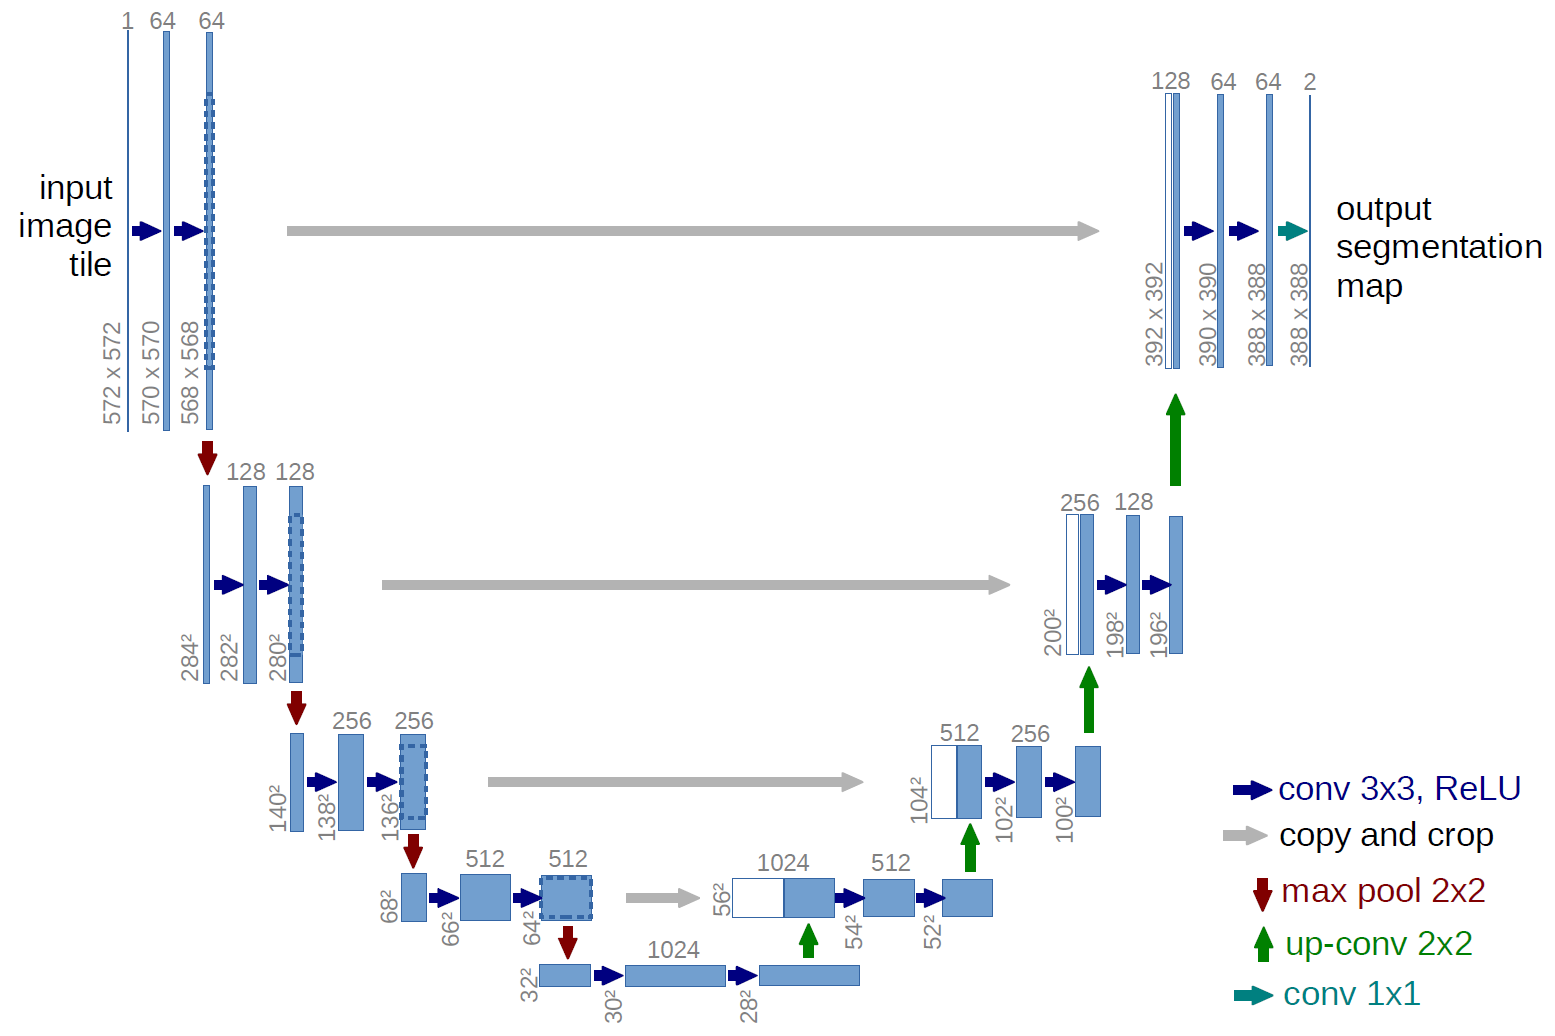
\includegraphics[width=1\textwidth]{images/background/latent_diffusion/u-net-architecture.png}
    \caption{Architecture of U-Net as introduced in the paper \cite{ronneberger2015unetconvolutionalnetworksbiomedical}.}
   \label{fig:U-Net}
\end{figure}


U-Net consists of four components: encoder, bottleneck, decoder, and skip-connections \cite{tai2024mathematicalexplanationunet}. The encoder is used to extract features, and its architecture is topologically identical to convolutional layers \cite{Liu2018ACL}. As max-pooling downsampling reduces the spatial dimensions of the image, the model can capture detailed and broad patterns, which are stored in feature maps for later use in the decoder. The bottleneck is the bottom layer of the U-shape that connects the encoder and decoder to transfer extracted features in their compressed representation. \cite{shah2024enhancingdiffusionmodelshighquality} The decoder reconstructs that compressed data by upsampling and using skip-connections. Skip-connections are used after each upsampling step to concatenate the deconvolved feature maps with feature maps from the corresponding part of the encoder. \cite{tai2024mathematicalexplanationunet, shah2024enhancingdiffusionmodelshighquality} In this way, U-Net can restore lost spatial information from downsampling and combine semantic information from the decoder with spatial information from the encoder, helping to connect features to the context \cite{liu2020holisticallyguideddecoderdeeprepresentation}.

%maybe telling about what is the output of the U-net in image segmentation and diffusion models.

%Neural network model learns the mean of the gaussian distribution of input image which is known as denoising score matching. 

\subsection{Transformers}
\label{sec:transformers}
Several popular modern AI applications, such as the large language model (LLM) ChatGPT and text-to-image model DALL-E, utilize transformer architecture. Transformers were proposed in 2017 by Vaswani et al. \cite{vaswani2023attentionneed} to address the limitations of traditional sequence-to-sequence models, whose operations are slow due to limited parallelization and which cannot capture relationships between elements in long-range dependencies, also known as the vanishing gradient problem. The main idea of transformers is to use a self-attention mechanism to capture relationships between all elements in the input sequence, which also enables parallel training. \cite{ISLAM2024122666} In this section, the focus will be on embedding vectors, self-attention, and cross-attention mechanisms, as they are important for understanding how they are used later in the chapter discussing latent diffusion models.

A standard transformer consists of two parts: an encoder and a decoder. The encoder processes and encodes the input sequence into a hidden space, while the decoder generates the target output based on the encoded representation. These two parts can also be used independently, resulting in encoder-only and decoder-only models. Encoder-only models, like BERT, are usually applied to tasks such as classification, regression, and ranking, while decoder-only models, like ChatGPT, are used for generative tasks and language modeling. \cite{fu2023decoderonlyencoderdecoderinterpretinglanguage, suganthan2025adaptingdecoderbasedlanguagemodels}

\begin{figure}[!h]
    \centering
    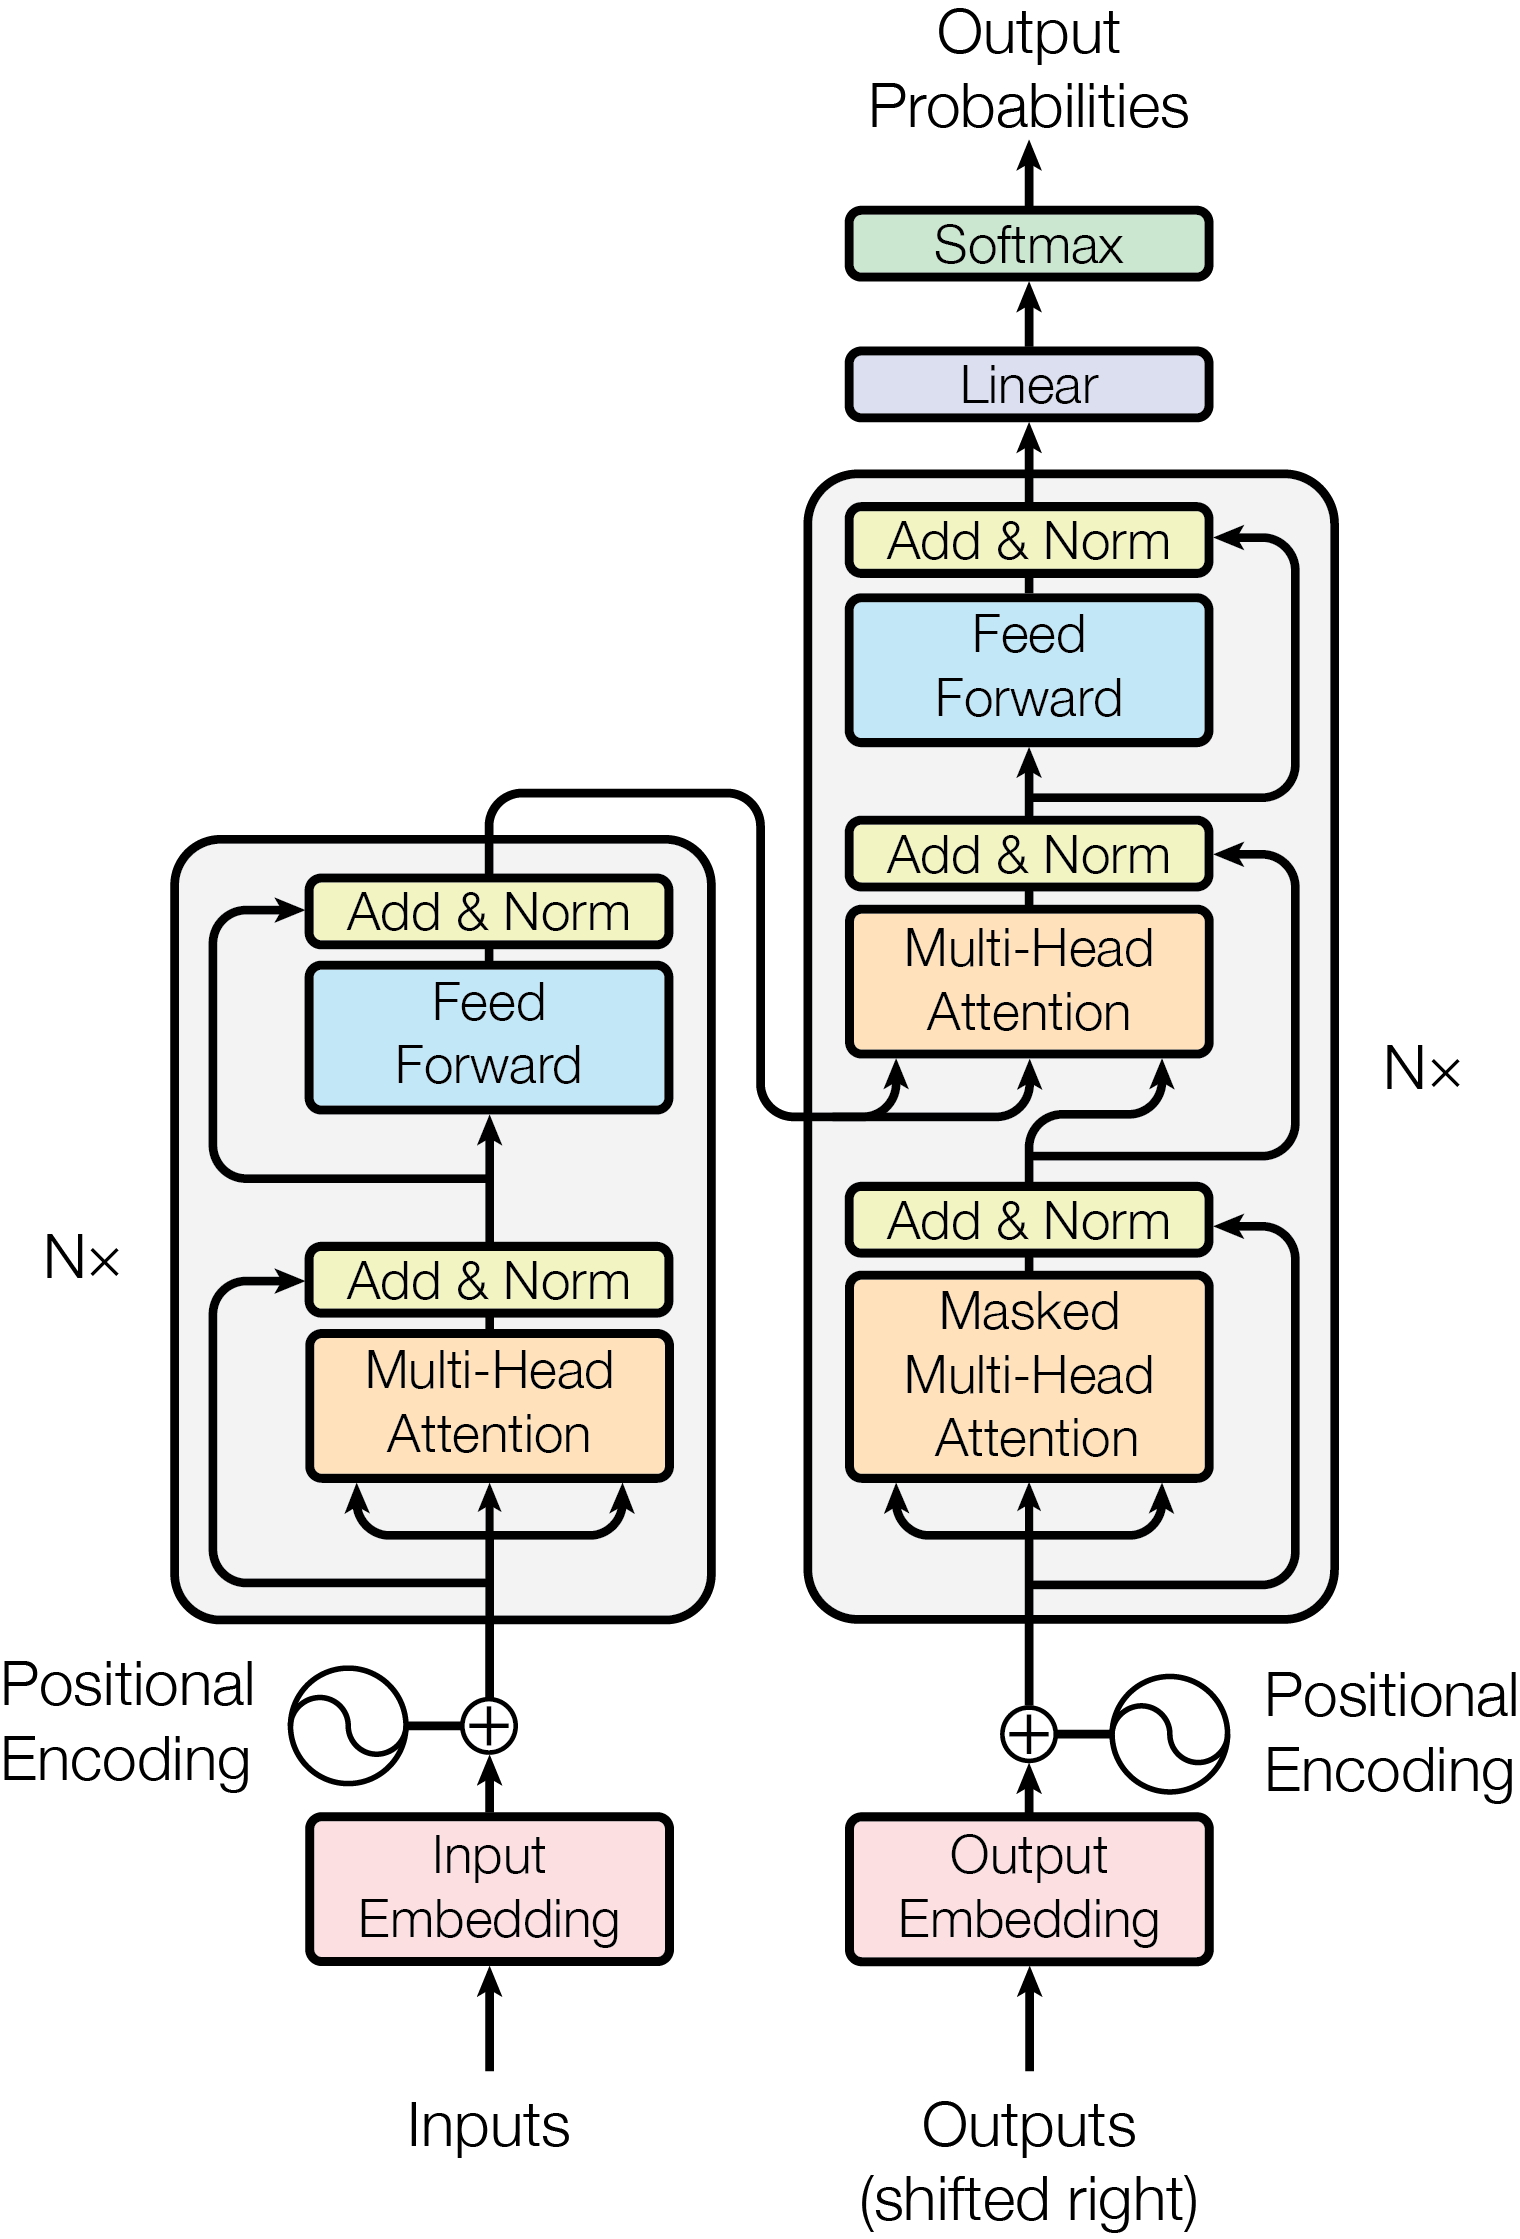
\includegraphics[width=0.6\textwidth]{images/background/latent_diffusion/ModalNet-21.png}
    \caption{Transformer architecture introduced in by Vaswani et al. 2017 \cite{vaswani2023attentionneed}.}
   \label{fig:Transformer}
\end{figure}

At the beginning of the transformer, input data is tokenized, meaning that the input data is divided into smaller parts. Depending on the type of input data, these can be patches of images, segments of an audio signal, or parts of words \cite{Susnato,Tnbeats}. Each token is then converted to a numerical vector called an embedding. These vectors are denoted as $E_i \in \mathbb{R}^{1 \times D}$, where $E$ is the index of a certain embedding and $D$ is the dimension of the embedding vector. The dimension $D$ is usually on the order of hundreds, but can be over ten thousand in large models like GPT-3.
Embedding vectors capture the semantic meaning and relationships of tokens in the embedding space, which can be measured with cosine similarity. In textual data, this means that words with similar meanings, like "car" and "motorcycle," are close to each other in the embedding space. Also, the vector distance between two embeddings can capture semantic information. For example, the distance between "France" and "Paris" is very similar to the distance between "Finland" and "Helsinki," encoding the "capital of" relationship. \cite{arsenievkoehler2021theoreticalfoundationslimitsword} However, polysemous words like "rock," which can mean stone or music genre depending on the surrounding words, can get their contextual meaning through the attention mechanism, where the initial embedding value is adjusted based on other embeddings in the sequence.

As embeddings themselves do not have any information about their relative position in the sequence, it is necessary to insert that information into the embedding by positional encoding. In \cite{vaswani2023attentionneed}, a sinusoidal function is used to capture positional information, which is injected into all elements of the embedding vector. Even though this information is added together with the embedding vector, the transformer will learn what is positional and what is semantic information in the embedding vector. There are many other ways to implement positional encoding, such as fixed or learned, and addition or concatenation, but they are outside the scope of this work. \cite{posen,kazemnejad2019}

The attention mechanism determines, for each embedding in the sequence, its relative importance to the other embeddings. When attention is applied to an embedding, it can increase or decrease the influence of the other embeddings, giving it contextual meaning over large distances in the sequence. In literature, it is said that the attention mechanism "attends to" other elements in the sequence, meaning it focuses on the most relevant parts of the input. \cite{vaswani2023attentionneed,Bergmann_Stryker_2025, 10049971} The main idea behind computing attention is based on three different vectors that are distinct representations of a single embedding vector: the query vector $Q_i$, the key vector $K_i$, and the value vector $V_i$ \cite{kowsher2025doesselfattentionneedseparate}. In plain language, these three vectors work together to produce attention as follows: the query asks which keys have important information for it; the keys contain information that is stored in the corresponding value vector and respond to the query about how important their information is. The attention mechanism computes weights that represent the importance of each value for the query. After the query receives these importance weights, it takes a weighted average of the information from the values, producing the attention output. This basic idea is behind many different types of attention mechanisms, such as self-attention and cross-attention. Next, it will be explained how self-attention computes attention and how it differs from cross-attention.

\begin{figure}[!h]
    \centering
    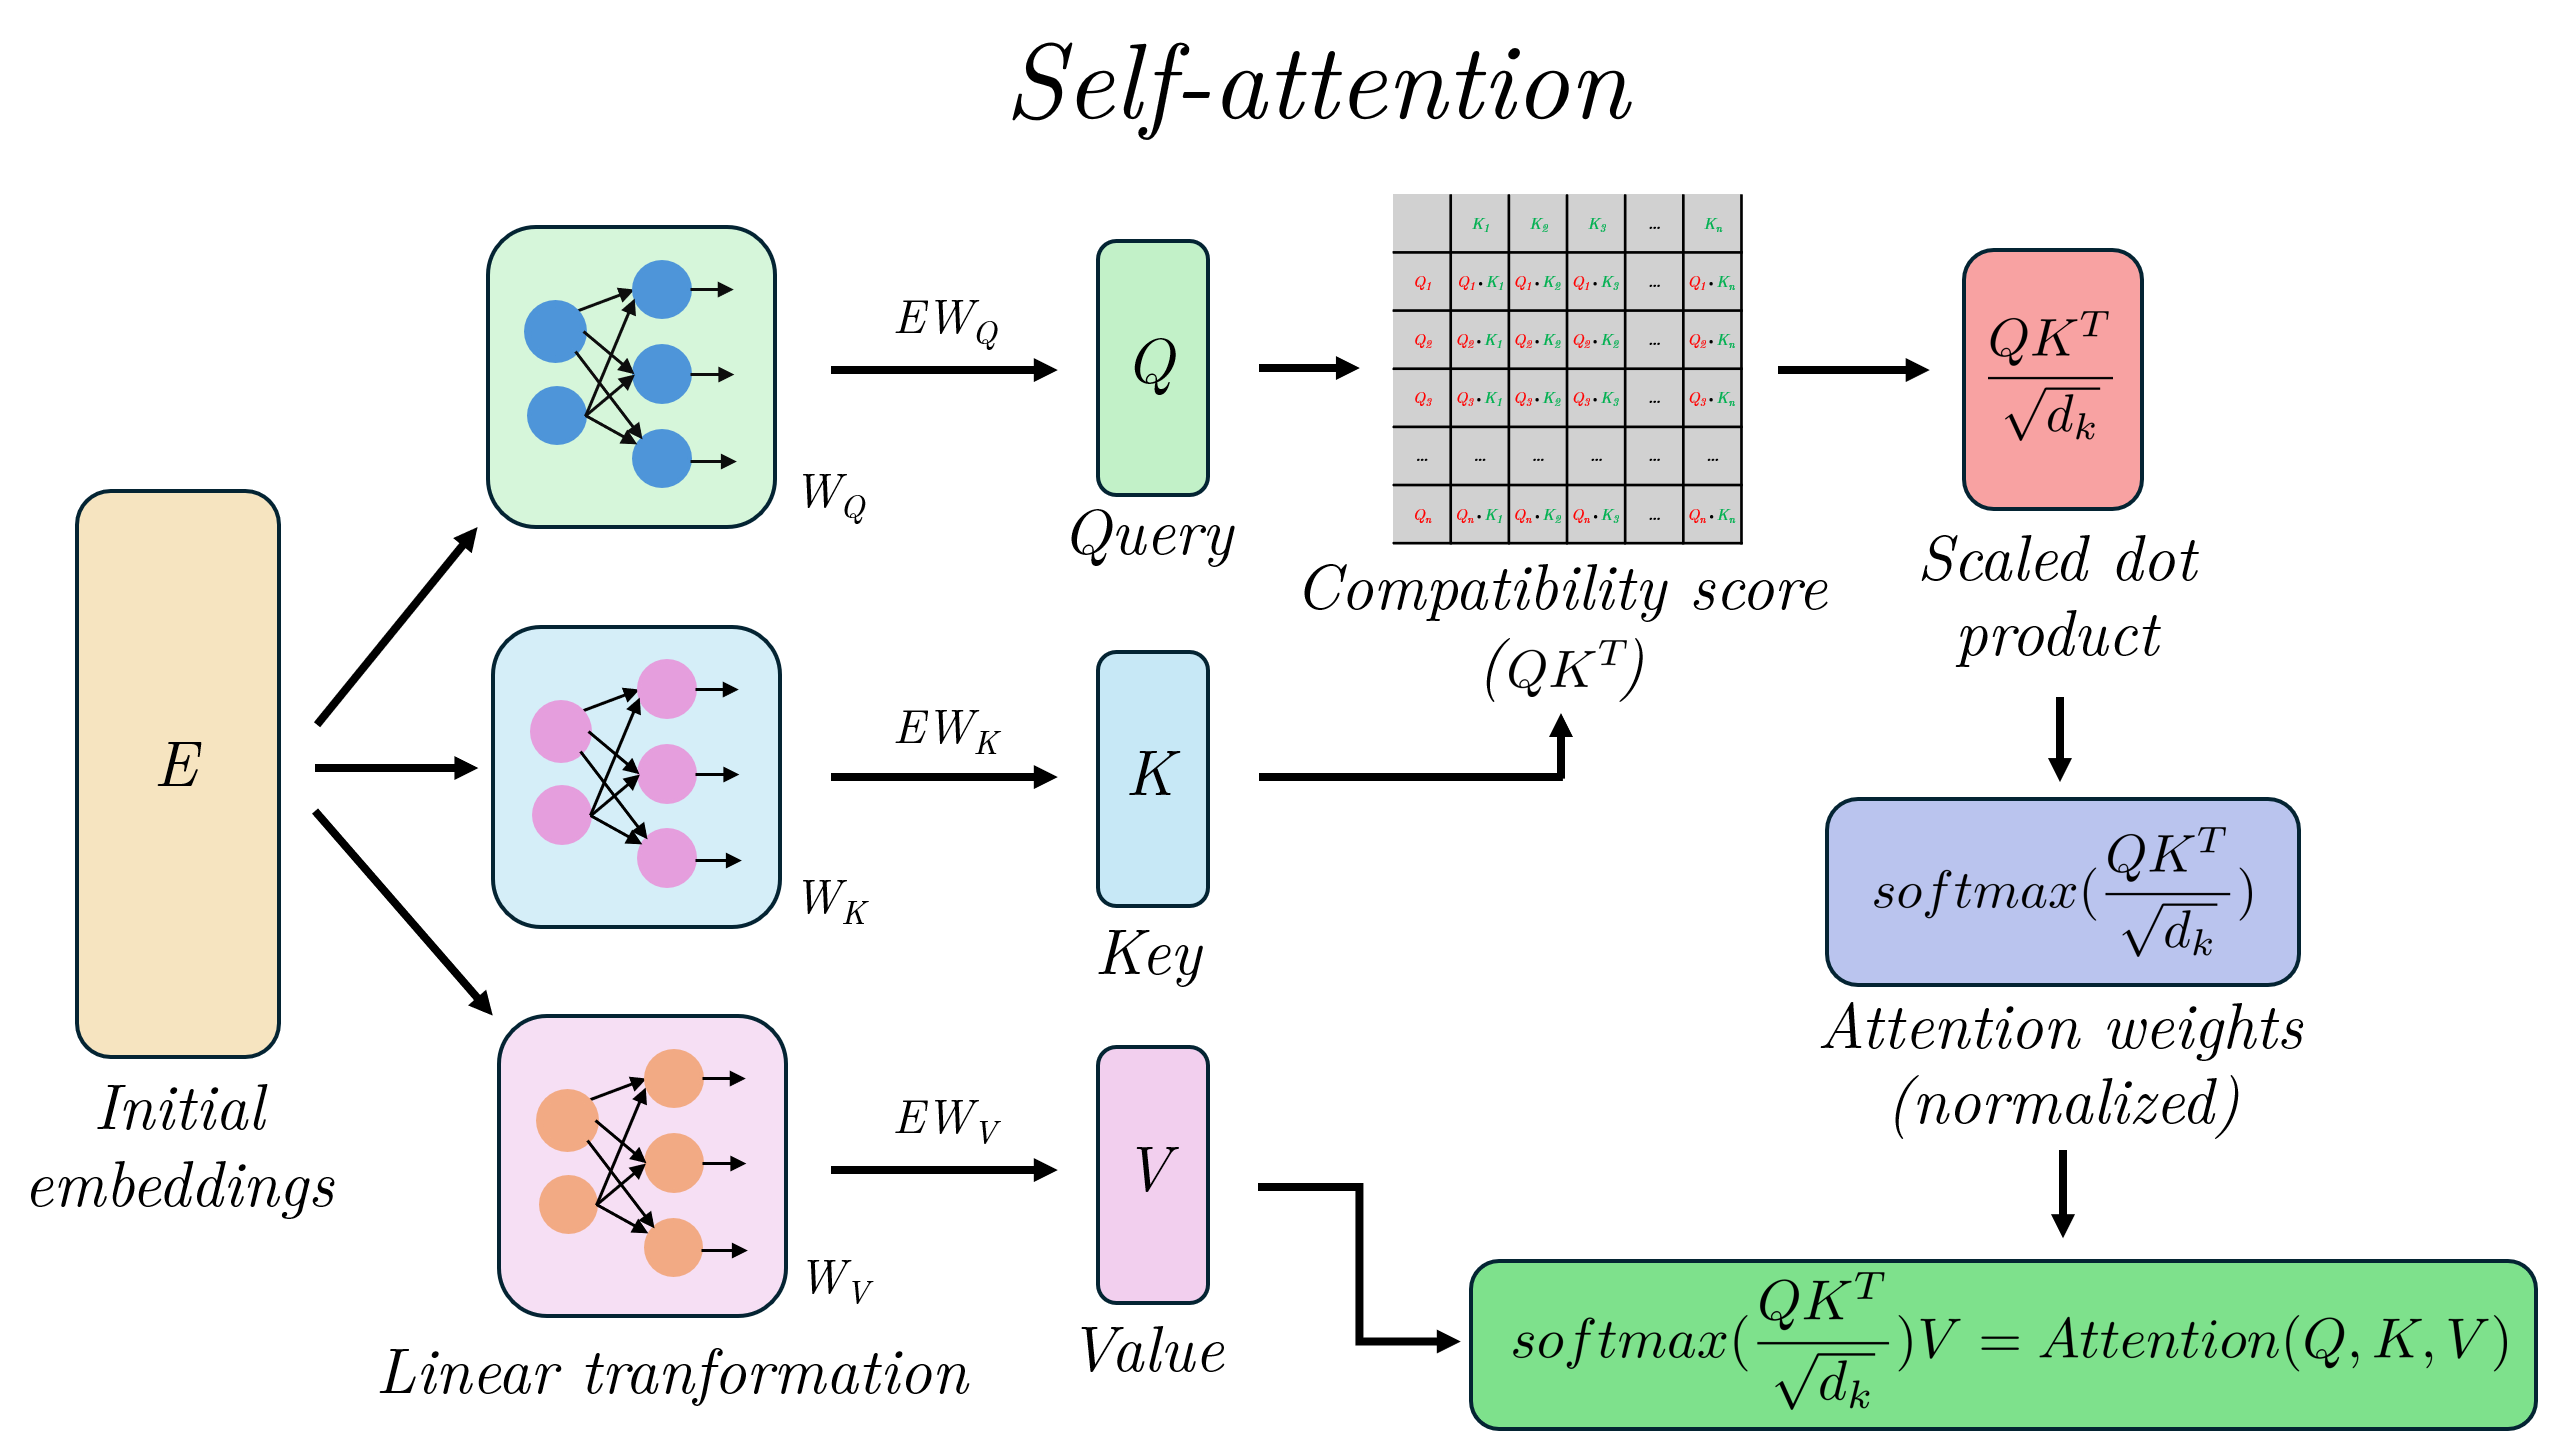
\includegraphics[width=1\textwidth]{images/background/CNN/Attention.PNG}
    \caption{The diagram about self-attention mechanism to calculate attention.}
   \label{fig:attention}
\end{figure}

In the self-attention mechanism, the embedding vector for each token is transformed into query, key, and value vectors. This is done by a linear transformation, i.e., multiplying the embedding vector with weight matrices $W_q$, $W_k$, and $W_v$ assigned for the query, key and value respectively. The weights of these matrices are learnable parameters\footnote{A single-layer neural network performs a linear transformation $y=Wx$ (purely linear transformation) or $y=Wx+b$ (affine linear transformation) when an activation function is not used.} that are the same for every embedding vector. \cite{transformerBERTGPT} The role of the weight matrices in the attention mechanism is to extract relevant features from the embedding that are important for their tasks. For $W_q$ and $W_k$, it is search, and for $W_v$, it is retrieval. \cite{mittal2022compositionalattentiondisentanglingsearch, Mehta2023TheAM} These linear transformations for all embeddings in the sequence can be expressed as:

\begin{equation}
    Q = E W_Q \,, \quad K = E W_K \,, \quad V = E W_V \,,
\end{equation}

where $E$ is the embedding matrix and $Q$, $K$ and $V$ are the query, key, and value in their matrix form. \cite{transformerBERTGPT} Once these matrices are calculated, the query and key matrices are used to create a compatibility score, which is the dot product between the query and key matrices ($QK^T$). This dot product is then scaled by dividing it by the square root of the dimension of the key vector $d_k$. Scaling is done to prevent the dot product from becoming too large, which could lead to vanishing gradients. In the next step, attention weights (also called attention scores) are computed by normalizing with softmax. \cite{bernhard2023alternativesscaleddotproduct} The computed attention weights are then multiplied with the value matrix:

\begin{equation}
    Attention(Q,K,V) = softmax\left(\frac{QK^T}{\sqrt{d_k}}\right)V \,,
\end{equation}

giving attention values that show how much each embedding attends to other embeddings. In transformers, multi-head attention is usually used, where multiple self-attention layers run in parallel. In the multi-head attention, each layer has its own distinct weight matrices, producing distinct attention values that are concatenated at the end. \cite{vaswani2023attentionneed}

Cross-attention is very similar to the self-attention mechanism. The most important difference between these two is that, in the cross-attention mechanism, input is taken from two different sources instead of one. In practice, in cross-attention, the key and value come from one dataset and the query comes from another dataset. This makes it possible to align two different modalities, such as image and text, speech and image, or EEG signal and speech. \cite{CLIP, 10191393, desilva2024neurospexneuroguidedspeakerextraction}

\section{Synthetic Data in Object Detection}
\label{sec:synthetic_data_object_detection}

The motivation to use synthetic data is mainly related to the difficulties of collecting large and diverse datasets for training object detection models \cite{voetman2023bigdatamythusing}. Common reasons for supplementing a dataset with synthetic data include an insufficient amount of real data, lack of public datasets, or the absence of pretrained models for similar use cases. In addition, capturing real data can have several challenges, such as high costs, time-consuming annotating, and privacy concerns. Synthetic data can help alleviate these challenges in training object detection models. \cite{kiefer2021leveragingsyntheticdataobject, Delussu2024synthetic, nguyen2024application}

\begin{figure}
    \centering
    \subcaptionbox{3D model-based synthesis \cite{tremblay2018trainingdeepnetworkssynthetic}}{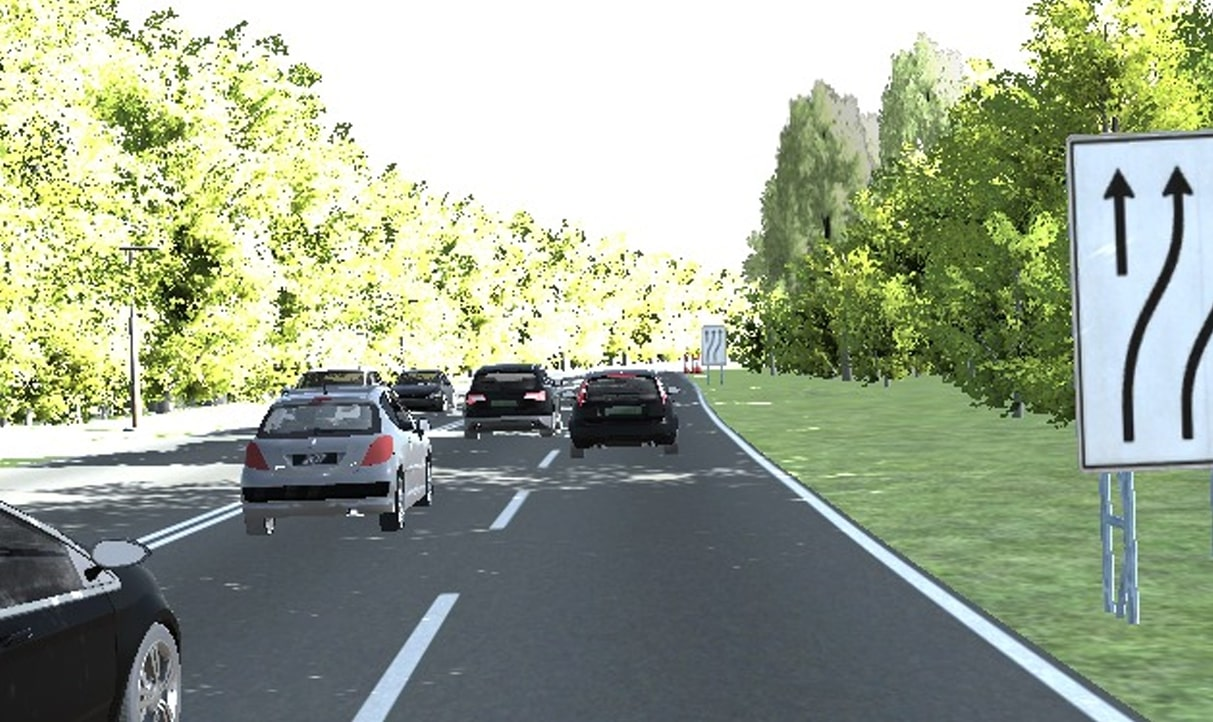
\includegraphics[height=8\baselineskip]{images/background/syn2img/3d2.jpg}} \quad
    \subcaptionbox{Text-to-image generation \cite{tang2024crsdiffcontrollableremotesensing}}{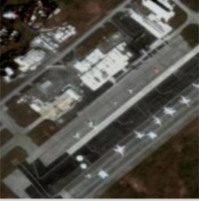
\includegraphics[height=8\baselineskip]{images/background/syn2img/aerial.PNG}} \quad
    \subcaptionbox{Image blending \cite{georgakis2017synthesizingtrainingdataobject}}{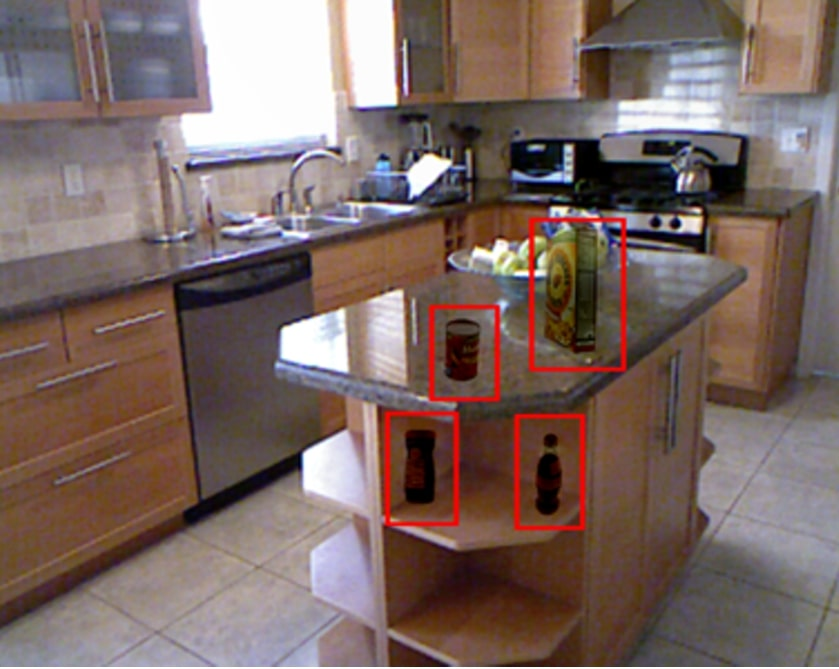
\includegraphics[height=8\baselineskip]{images/background/syn2img/blend.jpg}}\quad
    \caption{Different techniques to synthesize data for object detection training.}
    \label{fig:syn2real}
\end{figure}

The most common techniques to generate synthetic data are 3D model-based synthesis, text-to-image generation and image blending. For example, depending on the method used, synthetic data generation can quickly and cheaply produce large amounts of data and enable auto-labeling \cite{kiefer2021leveragingsyntheticdataobject, nguyen2024application}. Synthetic data generation methods also have the controllability to simulate rare scenarios and objects that do not appear in real datasets, making it possible to train models to detect edge cases \cite{Zhang2024, edgecases}. However, when only simulated or synthetic data is used to train object detection models for real-world applications, model performance is usually lower than when using real-world data for training. This happens because the input distribution has shifted between synthetic and real data. In the literature, this shift is commonly referred to as the synthetic-to-real (syn2real) or simulation-to-real (sim2real) gap. \cite{vanherle2022analysistrainingobjectdetection, mishra2024closingvisualsimtorealgap} To close this gap, there are different approaches that can be used to improve synthetic data generation. Next, reviewed papers are introduced in Table~\ref{tab:syn2realtable} that are related to the syn2real problem in the object detection field, where different techniques are used to generate synthetic data.

\begin{table}[h!]
        \caption{Summary of studies focusing on training object detection with synthetic data.}
            \label{tab:syn2realtable}
    \centering
    \scriptsize
    \renewcommand{\arraystretch}{1.1}
    \begin{threeparttable}
    \begin{tabular}{P{1.75cm}|P{2.5cm}|P{2.5cm}|P{1.85cm}|P{2.25cm}|P{1.25cm}}
    \hline
    \textbf{Technique} &
    \textbf{Study Focus} &
    \textbf{Synthetic Image Generation Method} &
    \textbf{\makecell[l]{Performed well \\ with synthetic \\ data only \tnote{1}}} &
    \textbf{\makecell[l]{Performed better \\ with synthetic \\ and real data \\ than only \\ using real data \tnote{2}}} &
    \textbf{Reference} \\ \hline \hline

    3D simulation & Arbitrary objects for robot perception & iPhone 3D scans and NVIDIA Omniverse Isaac Sim & Yes & - & \cite{singh2024syntheticalargescalesynthetic} \\ \hline
    3D simulation & Traffic vehicle detection & Domain randomization using 3D models & Yes & Yes & \cite{tremblay2018trainingdeepnetworkssynthetic} \\ \hline
    3D simulation and Text2img & Aerial ship detection & Unity and Stable Diffusion with different domain adaptation algorithms & - & - & \cite{app14114558} \\ \hline
    Image blending & Arbitrary objects in indoor scenes & Object placement and blending into real photos & No & Yes & \cite{georgakis2017synthesizingtrainingdataobject} \\ \hline
    Image blending & Milk package detection in refrigerator & Object placement and blending into real photos & No & Yes & \cite{Bartolovic2024FromST} \\ \hline
    Img2img & Aerial transmission tower and tower component detection & Synthesizing images using the AirSim simulator and Unreal Engine and adapting those to be more realistic using CycleGAN, CUT, and TSIT & Yes & Yes & \cite{Peterlevitz2023SimtoRealTF} \\ \hline
    Img2img & Industrial object detection & CycleGAN-based model with two generators and two discriminators & Yes & Yes & \cite{math11224588} \\ \hline
    Text2img & Aerial object detection & Fine-tuning Stable Diffusion model & No & Yes & \cite{jian2023stablediffusionaerialobject} \\ \hline
    Text2img & Downstream road detection & Fine-tuning Stable Diffusion model & Yes & Yes & \cite{tang2024crsdiffcontrollableremotesensing} \\ \hline
    Text2img & Heavy machinery detection and classification & DreamBooth framework with Stable Diffusion XL (SDXL) & No & Yes & \cite{xin2024dartautomatedendtoendobject} \\ \hline
    Text2img & Motorcyclists' helmet violation detection & Convolutional generative adversarial networks (DCGANs) & - & Yes & \cite{a17050202} \\ \hline
    Text2img & Skin disease classification & Stable Diffusion & Yes & Yes & \cite{akrout2023diffusionbaseddataaugmentationskin} \\ \hline
    Text2img & Traffic vehicle detection and classification in urban applications & Kandinsky 2.2 diffusion model & - & - & \cite{REUTOV2023335} \\ \hline
    Text2img & Underwater mine-like object detection & Comparison of synthetic data generation methods, including GANs and diffusion models (DDPM and DDIM) & Yes & Yes & \cite{agrawal2024syn2realdomaingeneralizationunderwater} \\ \hline
    \end{tabular}
    \begin{tablenotes}[para,flushleft]
    \footnotesize
    \item[1] \textbf{“Performed well with synthetic data only”} indicates the performance of a model trained solely on synthetic data. (“Yes”) = comparable performance; (“No”) = poor performance with mAP typically below 10\%; (“–”) = only trained with real or mixed data. \\
    \item[2] \textbf{“Performed better with synthetic and real data than only using real data”} indicates whether mixed data improved performance compared with using real data alone. (“–”) = only trained with synthetic or mixed data. \\
    \end{tablenotes}

    \end{threeparttable}
\end{table}

From Table~\ref{tab:syn2realtable}, it can be seen that most techniques achieved promising results even when using only synthetic data for training. However, some approaches performed poorly when synthetic data was used alone, likely due to a large gap between the synthetic and real domains. Despite this, all reviewed studies reported improved performance when mixed datasets were used compared to real data alone. This indicates that useful features can be extracted from synthetic data for training, even when the visual domains differ, as long as real data is also included in the training process. For example, \cite{georgakis2017synthesizingtrainingdataobject} found that a mixed dataset of 400 real and 20000 synthetic images outperformed a model trained with 5000 real images alone, while a fully synthetic training dataset produced poor results.

Across the reviewed papers, there were mainly two approaches to using synthetic data: (1) training the model only with synthetic data and then fine-tuning it with real data, or (2) training the model with both synthetic and real data simultaneously. In \cite{burdorf2022reducingrealworlddata}, no significant difference was found between these approaches. It was estimated that using a mixed dataset with 5\%-20\% real and 80\%-95\% synthetic data can reduce the amount of real data required without sacrificing performance \cite{burdorf2022reducingrealworlddata}. However, based on the literature, the optimal ratio appears to be case-dependent, as the effectiveness of synthetic data varies by task domain and generation technique.

Among the reviewed studies, synthetic data generation techniques can be broadly grouped into four categories, each with distinct advantages and limitations.

\textbf{3D simulation} techniques (e.g., NVIDIA Omniverse Isaac Sim, Unity) use simulation or game engines to create synthetic environments with controllable objects, cameras, and scene configurations. The realism of the simulation and the required time depend on various factors such as the quality of 3D models and rendering techniques. Different settings, such as object positions, viewpoints, and lighting, can be randomized to automatically produce diverse images. The generated images are usually labeled or segmented during the simulation process. Creating high-quality 3D assets can be time-consuming, especially if no pre-existing models are available.

\textbf{Image blending} techniques create synthetic images by inserting or blending object images into real backgrounds. Objects are typically cut from other images and placed into new backgrounds after defining suitable background surfaces and scaling the objects accordingly. Similar to 3D simulation, image blending methods can also use randomization to create diverse datasets and enable automatic labeling. A common limitation is that objects do not always visually blend well with the background. This may lead to poorer model performance when trained solely on blended images likely due to visual domain gaps (e.g., lighting inconsistencies) between synthetic and real components.

\textbf{Image-to-image (img2img) translation} techniques use deep learning–based generative models, such as CycleGAN or diffusion models, to translate images from a synthetic domain to a more realistic one. For example, images generated using 3D simulation or image blending can be adapted to appear more realistic through these methods. Well-trained img2img models can produce high-quality and diverse images, typically improving object detection performance compared to using only synthetic data. The required workload depends on whether suitable synthetic images already exist or need to be created first.

\textbf{Text-to-image (txt2img) generation} techniques are similar to img2img methods, but instead of using synthetic images as input, they are trained on datasets containing images paired with textual descriptions. This allows the generation of a wide variety of images using text prompts, enabling control over factors such as object type, lighting, and quantity. By fine-tuning a pre-trained base model trained on large-scale datasets, it is possible to generate images that closely resemble a target real-world dataset. A drawback is that the generated images usually require manual annotation to label objects for object detection training.

Overall, text-to-image methods, such as Generative Adversarial Networks (GANs) and diffusion models, have shown the greatest potential for generating realistic and diverse data for object detection. A systematic review by \cite{Balance} similarly concluded that these models have strong potential to overcome sim2real problems.

For this work, it was decided to use diffusion-based text-to-image generation, specifically Stable Diffusion XL (SDXL), to generate synthetic training data for object detection model development, for the following reasons:

\begin{itemize}
\item \textbf{High-fidelity image generation:} SDXL can effectively learn the data distribution of real datasets and generate images with similar visual characteristics.
\item \textbf{Controllability:} The model enables control of image content through text prompts, allowing targeted dataset creation. Prompts can also be randomized to increase diversity in the generated data.
\item \textbf{Practical advantages:} SDXL is an open-source text-to-image model based on an improved version of Stable Diffusion v1.5 and is supported by fine-tuning tools. It also offers relatively fast image generation, depending on the GPU used, and has a large community providing numerous guides and tips.
\item \textbf{Rapid model evolution:} Text-to-image models have evolved significantly in a short time and continue to improve, making them strong candidates for future synthetic data generation.
\item \textbf{Integration with image-to-image tools:} SDXL can be adapted with techniques such as ControlNet (see Section~\ref{sec:conditioning}) to modify or guide generation according to input images. This can be useful for future works such as transforming standard photos into sensor-like images.
\end{itemize}

In following sections provide more information about text-to-image models, diffusion models, Stable Diffusion, and fine-tuning with Low-Rank Adaptation (LoRA).


\section{Text-To-Image Models}

Text-to-image (T2I) models generate images from textual descriptions, combining the fields of computer vision and natural language processing \cite{diffusionmodelssurvey, T2Isurvey}. The main goal of these models is to create new, high-quality images, rather than retrieving existing ones using textual conditioning. Modern T2I models are capable of producing images with strong text-image consistency and can handle complex prompts by large-scale training on millions of image-text pairs. \cite{T2Isurvey}

\begin{figure}[!h]
    \centering
    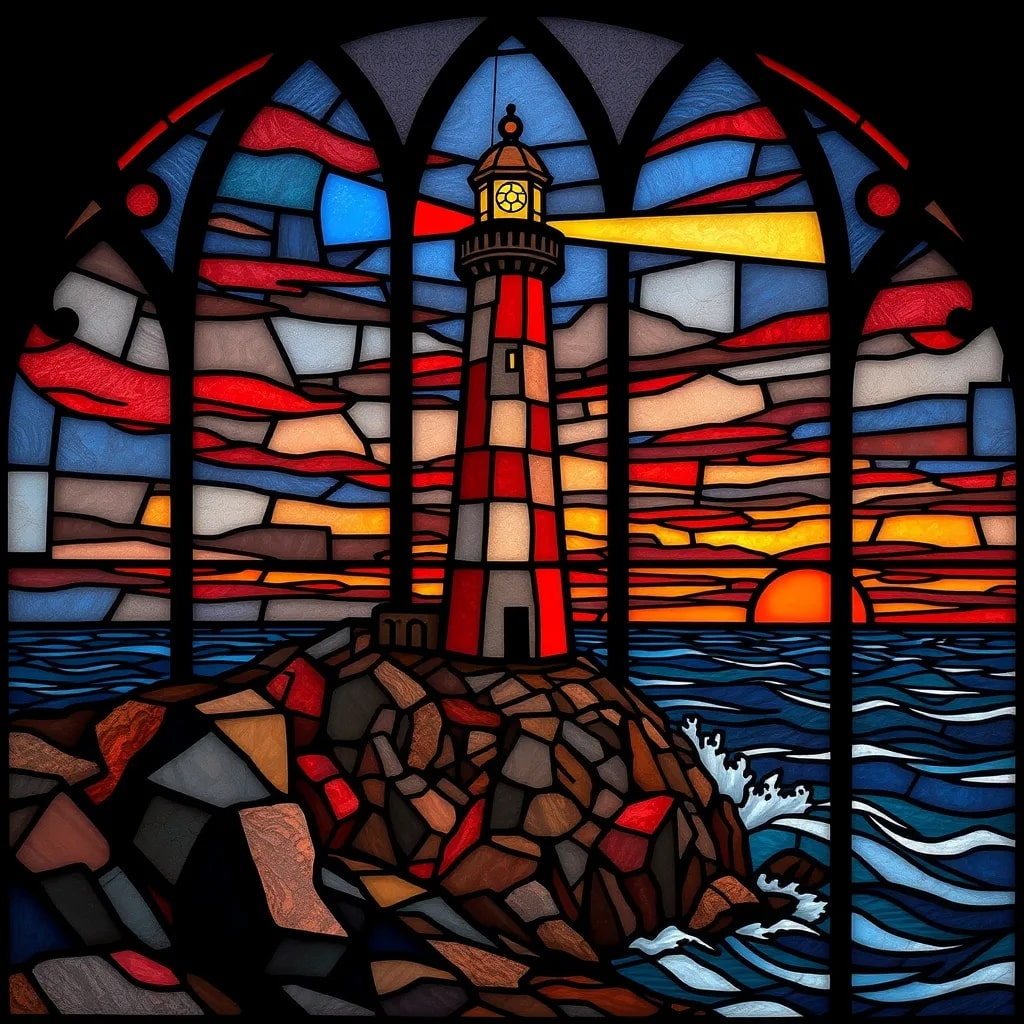
\includegraphics[width=0.5\textwidth]{images/background/txt2img/kuva.jpg}
    \caption{Generated image from FLUX.1 [schnell] using prompt "Gothic stained-glass of a lighthouse standing at the end of a rocky coast beside a wavy ocean under a red dawn sky."}
   \label{fig:t2i_timeline}
\end{figure}

The modern development of T2I models began in 2015 with AlignDRAW, which demonstrated the relationship between text input and generated images using attention mechanisms, although the results were not very realistic \cite{diffusionmodelssurvey, T2Isurvey}. After 2015, T2I made a great leap forward with Generative Adversarial Networks (GANs), leading to better image generation. In 2021, OpenAI introduced DALL-E, an autoregressive (AR) model that used transformer architecture and large-scale datasets to generate diverse, high-quality images, even though it suffered from high computational costs.\cite{T2Isurvey} In recent years, diffusion models (DM), such as DALL-E 2 and FLUX.1, have become the leading approach in T2I generation. Latent diffusion models (LDM), which are used for example in the Stable Diffusion models, not only improve the quality of generated images but also reduce computational costs by operating in latent space instead of pixel space.\cite{diffusionmodelssurvey, T2Isurvey} There are still many challenges in T2I models, such as fine-grained control, contextual understanding, or accurately capturing spatial relationships described in text prompts \cite{T2Isurvey}.

This work will next focus on diffusion-based T2I models including latent diffusion models and stable diffusion XL. Further details on GANs or AR models can be found in \cite{T2Isurvey}.

%hybrids?
%multimodal models?
%https://www.linkedin.com/pulse/revolutionizing-image-generation-power-ethics-models-sheikhansari
\section{Diffusion Models and Stable Diffusion}
This section is divided into two main parts. The first two subsections present the theoretical foundations of diffusion-based text-to-image models, while the later subsections focus on Stable Diffusion, a latent diffusion model, and its fine-tuning with Low-Rank Adaptation. Since the training of latent diffusion models is heavily based on Denoising Diffusion Probabilistic Models (DDPM), the first subsection focuses on this perspective, based mainly on \cite{ho2020denoisingdiffusionprobabilisticmodels, strümke2023lecturenotesprobabilisticdiffusion}, while excluding other diffusion models such as Denoising Diffusion Implicit Models (DDIM).

\subsection{Diffusion Models}
Diffusion models (DM), also known as diffusion probabilistic models, are a type of generative model that uses a Markov chain to convert a distribution into the target data distribution through a diffusion process. In this context, that means converting an original complex image distribution to a simple standard Gaussian distribution and vice versa. In the forward process (also known as the diffusion process), Gaussian noise is added iteratively to the data at each step until the data is completely noisy. The goal of diffusion models is to learn how to reverse the forward process for sample generation, gradually reducing noise with each step. \cite{strümke2023lecturenotesprobabilisticdiffusion,sohldickstein2015deepunsupervisedlearningusing} The illustration of forward and reverse processes are shown in Figure~\ref{fig:diffusion_process}.

\begin{figure}[!h]
    \centering
    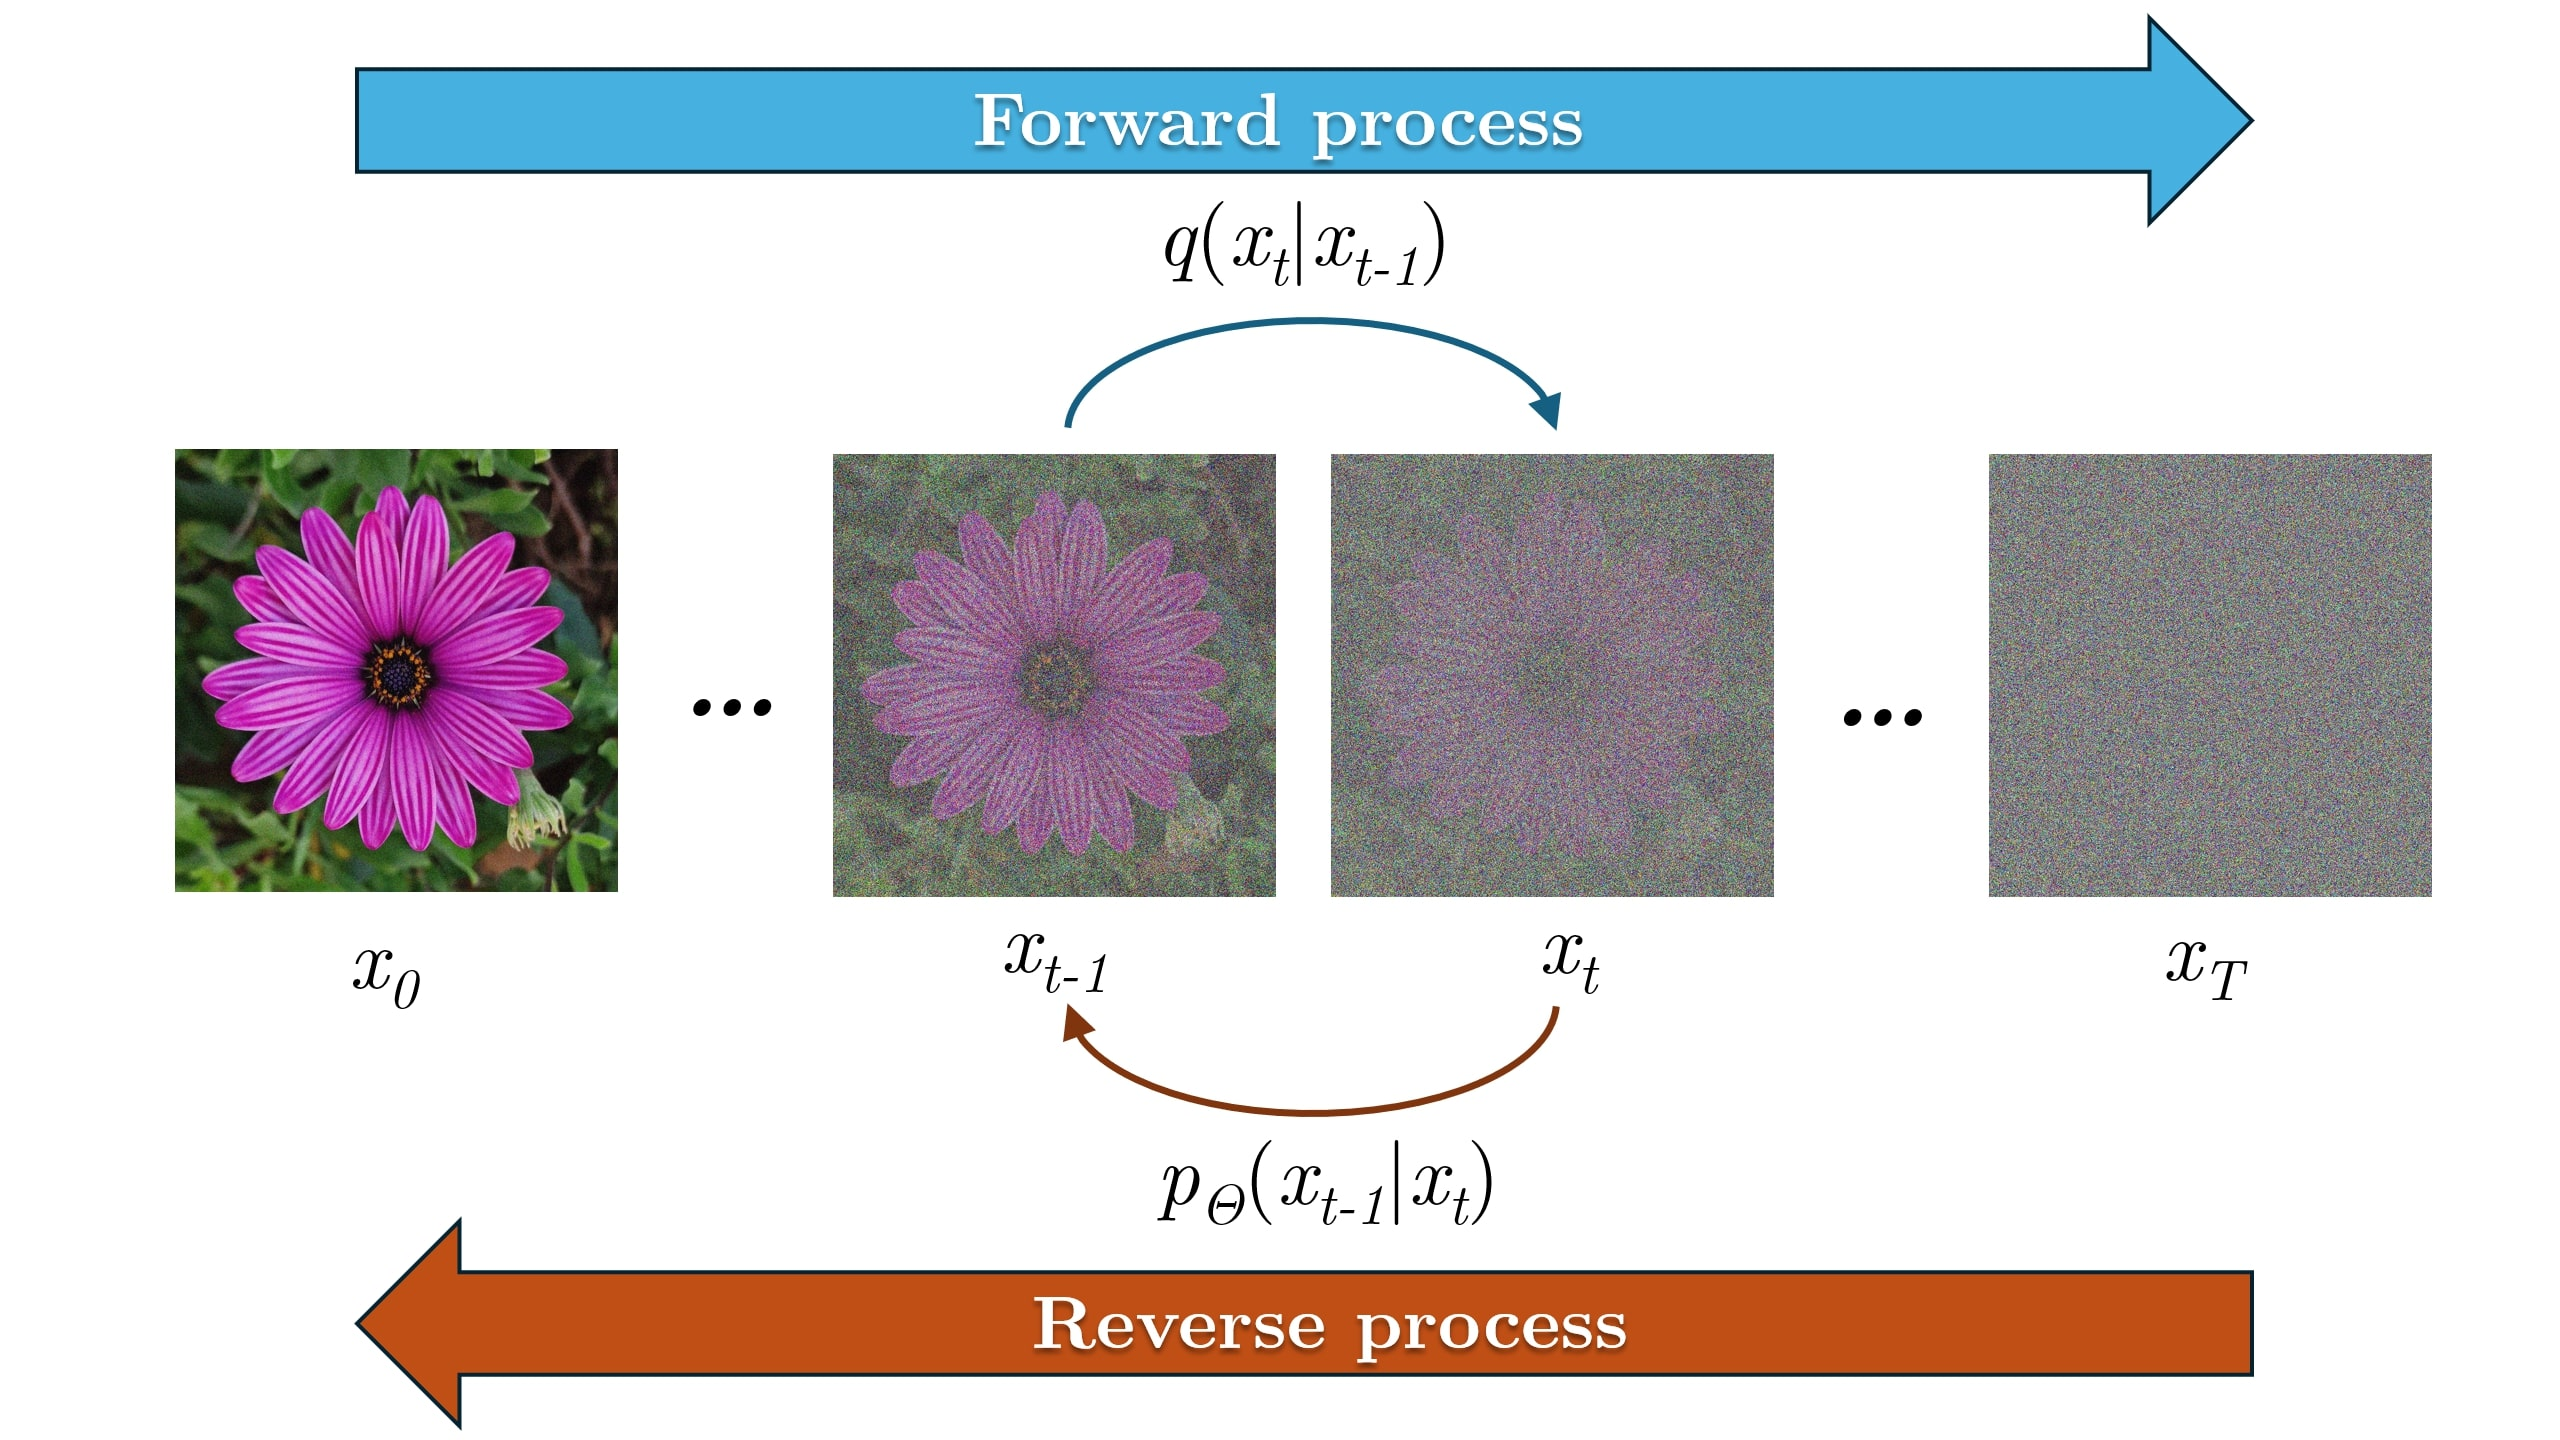
\includegraphics[width=1\textwidth]{images/background/latent_diffusion/diffusion_process.jpg}
    \caption{Forward and reverse processes in a diffusion model.}
   \label{fig:diffusion_process}
\end{figure}

{\textbf{Forward process}}

The forward process starts by providing a clean input data sample $\mathbf{x}_0$. This continues by adding standard Gaussian noise $\boldsymbol{\epsilon} \sim \mathcal{N}(0,\mathbf{I})$ at each time step, resulting in a noised sample $\mathbf{x}_t$ at time step $t$. The forward process ends at the last time step $T$, where the data is completely Gaussian noise. \cite{strümke2023lecturenotesprobabilisticdiffusion} The amount of Gaussian noise added to the sample at each step is determined by the variance schedule $\beta_1, \dots, \beta_T$, where the forward process variance $\beta_t$ (also referred to as the diffusion rate) can be precomputed, for example, by using a cosine noise scheduler, or can be learned \cite{shah2024enhancingdiffusionmodelshighquality,dellamaggiora2024conditionalvariationaldiffusionmodels}. Entire forward process from $\mathbf{x}_0$ to $\mathbf{x}_T$ can be written as joint probability

\begin{equation}
    q\left(\mathbf{x}_{1: T} \mid \mathbf{x}_{0}\right)=\prod_{t=1}^{T} q\left(\mathbf{x}_{t} \mid \mathbf{x}_{t-1}\right) \,,
    \label{eq:forward_process}
    \end{equation}
where $q$ denotes the probability distribution of the forward process. The noise added gradually at each step in \ref{eq:forward_process} can be written as

\begin{equation}
    q\left(\mathbf{x}_{t} \mid \mathbf{x}_{t-1}\right) = K \left(\mathbf{x}_{t} \mid \mathbf{x}_{t-1} ; \beta_{t}\right) \,,
    \label{eq:forward_process_step}
    \end{equation}
where $K$ is the Markov diffusion kernel, i.e. the sample $\mathbf{x}_t$ is generated from the previous sample $\mathbf{x}_{t-1}$. This also shows that as each diffusion step depends only on the previous step, the process is Markovian. \cite{strümke2023lecturenotesprobabilisticdiffusion}

When a Gaussian Markov diffusion kernel is used, the process is referred to as Gaussian diffusion. In this case, each forward process step is defined as a Gaussian distribution, and \ref{eq:forward_process_step} becomes

\begin{equation}
    q\left(\mathbf{x}_{t} \mid \mathbf{x}_{t-1}\right)=\mathcal{N}\left(\mathbf{x}_{t} ; \sqrt{1-\beta_{t}} \mathbf{x}_{t-1}, \beta_{t} \mathbf{I}\right) \,,
    \label{eq:forward_process_step_gaussian}
\end{equation}

where in the Gaussian distribution $\mathcal{N}$ the output is $\mathbf{x}_t$, the mean is $\sqrt{1-\beta_{t}} \mathbf{x}_{t-1}$, and the covariance matrix is $\beta_{t}\mathbf{I}$. \cite{strümke2023lecturenotesprobabilisticdiffusion,sohldickstein2015deepunsupervisedlearningusing}

To obtain the closed-form of equation \ref{eq:forward_process_step_gaussian}, let's introduce the reparametrization trick, where a Gaussian distribution $\mathbf{z} \sim \mathcal{N}(\mathbf{z}; \mu, \boldsymbol{\Sigma})$ can be defined as: 

\begin{equation}
\mathbf{z} = \mu + \mathbf{A}\boldsymbol{\epsilon}, \quad \boldsymbol{\epsilon} \sim \mathcal{N}(0,\mathbf{I}) \,,
\label{eq:reparametrization_trick}
\end{equation}
where $\mathbf{A}$ is such that $\boldsymbol{\Sigma} = \mathbf{A}\mathbf{A}^T$. By using the reparametrization trick, equation \ref{eq:forward_process_step_gaussian} can be written as

\begin{equation}
    \mathbf{x}_t = \sqrt{1-\beta_{t}} \mathbf{x}_{t-1} + \sqrt{\beta_{t}} \boldsymbol{\epsilon}_t \,.
    \label{eq:forward_process_step_reparametrization} 
\end{equation}

By defining signal retention rate $\alpha_{t}:=1-\beta_{t}$ and $\bar{\alpha}_{t}:=\prod_{s=1}^{t} \alpha_{s}$, equation \ref{eq:forward_process_step_reparametrization} can be derived to the following closed-form:

\begin{equation}
    \mathbf{x}_t = \sqrt{\bar{\alpha}_t} \mathbf{x}_0+\sqrt{1-\bar{\alpha}_t} \boldsymbol{\epsilon} \,,
    \label{eq:forward_process_step_closed_form}
\end{equation}

which can also be presented in a conditional Gaussian distribution form as

\begin{equation}
    q\left(\mathbf{x}_t \mid \mathbf{x}_0\right)=\mathcal{N}\left(\mathbf{x}_t; \sqrt{\bar{\alpha}_t} \mathbf{x}_0,\left(1-\bar{\alpha}_t\right) \mathbf{I}\right) \,.  
    \label{eq:forward_process_step_closed_form_gaussian}
    \end{equation}

As seen in equation \ref{eq:forward_process_step_closed_form}, $\mathbf{x}_t$ depends only on $\mathbf{x}_0$, so the sample $\mathbf{x}_t$ can be calculated directly, which makes the forward process fast.
The detailed derivation from equation \ref{eq:forward_process_step_reparametrization} to equation \ref{eq:forward_process_step_closed_form}, as well as other steps of the forward process, can be found in \cite{strümke2023lecturenotesprobabilisticdiffusion}. 

{\textbf{Reverse Process}}

To sample a clean image $\mathbf{x}_0$ from noisy data, the reverse process is required to gradually remove noise from a sample $\mathbf{x}_t$, producing reconstructed data samples. Like the forward process, the reverse process is a Markov chain, and the joint distribution of the whole reverse process can be written as

\begin{equation}
    p_{\boldsymbol{\theta}}\left(\mathbf{x}_{0: T}\right)=p(\mathbf{x}_T) \prod_{t=1}^{T} p_{\boldsymbol{\theta}}\left(\mathbf{x}_{t-1} \mid \mathbf{x}_{t}\right) \,,
    \label{eq:reverse_process}
\end{equation}

where $p$ is the probability distribution of the reverse process and $\boldsymbol{\theta}$ are the parameters of the neural network, as the reverse process needs to be learned. This is because $q(\mathbf{x}_{t-1}|\mathbf{x}_t)$ cannot be used for the noise reversal process guiding $\mathbf{x}_T$ back to $\mathbf{x}_0$, as it is intractable. This can be seen by using Bayes' rule to calculate $q(\mathbf{x}_{t-1}|\mathbf{x}_t)$ from $q(\mathbf{x}_t|\mathbf{x}_{t-1})$.\footnote{$q(\mathbf{x}_{t-1}|\mathbf{x}_t) = \frac{q(\mathbf{x}_t|\mathbf{x}_{t-1})q(\mathbf{x}_{t-1})}{q(\mathbf{x}_t)}$} As $q(\mathbf{x}_{t-1})$ and $q(\mathbf{x}_t)$ are not accessible, expanding these terms requires representing and integrating over the distribution $q(\mathbf{x}_0)$. That is not feasible, as the distribution of the original sample $\mathbf{x}_0$ is not assumed to be Gaussian but a complex distribution. This concludes that $q(\mathbf{x}_{t-1}|\mathbf{x}_t)$ cannot be calculated directly. \cite{strümke2023lecturenotesprobabilisticdiffusion}

Nonetheless, it is possible to approximate $q(\mathbf{x}_{t-1}|\mathbf{x}_t)$ by defining a new distribution to represent the reverse process. As the reverse step is also assumed to be Gaussian like the forward step, it can be written as

\begin{equation}
    p_{\boldsymbol{\theta}}\left(\mathbf{x}_{t-1} \mid \mathbf{x}_t\right)=\mathcal{N}\left(\mathbf{x}_{t-1} ; \boldsymbol{\mu}_{\boldsymbol{\theta}}\left(\mathbf{x}_t, t\right), \boldsymbol{\Sigma}_{\boldsymbol{\theta}}\left(\mathbf{x}_t, t\right)\right) \,. 
    \label{eq:reverse_process_step}
\end{equation}

Based on this, to learn equation \ref{eq:reverse_process_step} and thus produce the reverse step, it is necessary to estimate the mean and variance. In practice, as this work follows the implementation of DDPM from paper \cite{ho2020denoisingdiffusionprobabilisticmodels}, where the forward process variance $\beta_t$ is fixed, only the mean $\boldsymbol{\mu}_{\boldsymbol{\theta}}\left(\mathbf{x}_t, t\right)$ needs to be learned. In the referenced paper, it was empirically found that fixing the reverse-process variance as $\boldsymbol{\Sigma}_{\boldsymbol{\theta}}\left(\mathbf{x}_t, t\right) = \sigma_t^2 \mathbf{I}$ gives similar results whether the forward process variance $\sigma_t^2=\beta_t$ or the forward process posterior variance $\sigma_t^2=\tilde{\beta}_t$ is used (the latter will be derived later from the forward-process posterior $q(\mathbf{x}_{t-1}|\mathbf{x}_t,\mathbf{x}_0)$). Because of this, it was not specified separately whether variance was used for sampling algorithm at the end of this sections.

The next objective is to define the loss function to train the neural network to estimate the mean and then use that to derive the equation to sample $\mathbf{x}_{t-1}$ from $\mathbf{x}_t$. To define the loss function, it is intuitive to maximize the likelihood of $\mathbf{x}_0$, as generative models usually learn data distributions from training data. However, it is not possible to maximize the likelihood $p_{\boldsymbol{\theta}}\left(\mathbf{x}_0\right)$ directly, as calculating it involves integrating over all trajectories from $\mathbf{x}_T$ to $\mathbf{x}_0$, which is intractable. To circumvent this problem, it is possible to optimize an evidence lower bound (ELBO, also known as the variational lower bound) of the log likelihood\footnote{It is usually easier to work with log likelihood instead of maximizing likelihood, as it has various good properties such as being a monotonically increasing function, and maximizing the log also means maximizing the likelihood. Also, log likelihood turns multiplications into additions, making derivatives and sums easier to calculate.}, which is tractable. \cite{strümke2023lecturenotesprobabilisticdiffusion}

Equations after this point will follow paper \cite{ho2020denoisingdiffusionprobabilisticmodels}, which minimizes the ELBO of negative log likelihood instead of maximizing it.\footnote{While this work uses negative log likelihood, some papers may use positive log likelihood instead, like in paper \cite{sohldickstein2015deepunsupervisedlearningusing}. This is because maximizing log likelihood is equivalent to minimizing negative log likelihood. In that case, equation \ref{eq:loss} becomes $L := \mathbb{E}\left[\log p_{\boldsymbol{\theta}}\left(\mathbf{x}_0\right)\right] \geq \mathbb{E}_{q}\left[\log\frac{p_{\boldsymbol{\theta}}\left( \mathbf{x}_{0:T}\right)}{q\left( \mathbf{x}_{1:T} | \mathbf{x}_0\right)} \right]$}

The loss function $L$ is defined by minimizing the ELBO of the log likelihood as
\begin{equation}
L := \mathbb{E}\left[-\log p_{\boldsymbol{\theta}}\left(\mathbf{x}_0\right)\right] \leq \mathbb{E}_{q}\left[-\log\frac{p_{\boldsymbol{\theta}}\left( \mathbf{x}_{0:T}\right)}{q\left( \mathbf{x}_{1:T} | \mathbf{x}_0\right)} \right] \,,
\label{eq:loss}
\end{equation}

where $\mathbb{E}$ is the expectation operator. Next, the full derivation of the loss presented in \cite{ho2020denoisingdiffusionprobabilisticmodels} is omitted due to its length, and only the resulting loss function is presented:

\begin{align}
L = \mathbb{E}_q\Big[ 
    &\underbrace{D_{\mathrm{KL}}\left(q\left(\mathbf{x}_T \mid \mathbf{x}_0\right) \| p\left(\mathbf{x}_T\right)\right)}_{L_T} \notag \\
    &+ \sum_{t>1} \underbrace{D_{\mathrm{KL}}\left(q\left(\mathbf{x}_{t-1} \mid \mathbf{x}_t, \mathbf{x}_0\right) \| p_{\boldsymbol{\theta}}\left(\mathbf{x}_{t-1} \mid \mathbf{x}_t\right)\right)}_{L_{t-1}} \notag \\
    &\underbrace{-\log p_{\boldsymbol{\theta}}\left(\mathbf{x}_0 \mid \mathbf{x}_1\right)}_{L_0}
\Big] \,,
\label{eq:elbo_loss}
\end{align}

where $D_{\mathrm{KL}}$ is the Kullback-Leibler divergence\footnote{$D_{\mathrm{KL}}(P \| Q) = \sum_{} P(x) \log \frac{P(x)}{Q(x)}$}. In expectation, the loss is divided into three terms: the prior matching term $L_T$, the consistency term $L_{t-1}$, and the reconstruction term $L_0$. In \cite{ho2020denoisingdiffusionprobabilisticmodels}, the term $L_T$ is treated as a constant because $p(\mathbf{x}_T)$ is just Gaussian noise and a fixed forward process variance $\beta_t$ is used. As a result, the forward process distribution $q$ has no learnable parameters. The term $L_0$ is also ignored, as empirical testing showed that leaving it out not only simplifies the implementation of the loss function but also improves sample quality. This leaves only $L_{t-1}$ to be optimized.

To expand $L_{t-1}$, the forward process posterior $q(\mathbf{x}_{t-1}|\mathbf{x}_t,\mathbf{x}_0)$ needs to be defined as a Gaussian distribution. It can be calculated using Bayes' rule:

\begin{equation}
q(\mathbf{x}_{t-1} \mid \mathbf{x}_t, \mathbf{x}_0) = \frac{q(\mathbf{x}_t \mid \mathbf{x}_{t-1}, \mathbf{x}_0) \, q(\mathbf{x}_{t-1} \mid \mathbf{x}_0)}{q(\mathbf{x}_t \mid \mathbf{x}_0)} \,.
\label{eq:posterior_bayes}
\end{equation}

By utilizing the Markov property of the entire forward process $q(\mathbf{x}_{1:T}|\mathbf{x}_0)$\footnote{$q(\mathbf{x}_{1:T}|\mathbf{x}_0)= \prod_{t=1}^{T} q(\mathbf{x}_t|\mathbf{x}_{t-1}) = q(\mathbf{x}_T|\mathbf{x}_0) \prod_{t=2}^{T} q(\mathbf{x}_{t-1}|\mathbf{x}_t,\mathbf{x}_0)$}, it is obtained that $q(\mathbf{x}_t|\mathbf{x}_{t-1},\mathbf{x}_0) = q(\mathbf{x}_t|\mathbf{x}_{t-1})$, which is expressed in Gaussian form in equation \ref{eq:forward_process_step_gaussian}. Additionally, the Gaussian forms of $q(\mathbf{x}_{t-1} \mid \mathbf{x}_0)$ and $q(\mathbf{x}_t \mid \mathbf{x}_0)$ can be defined from equation \ref{eq:forward_process_step_closed_form_gaussian}, which now gives

\begin{equation}
q(\mathbf{x}_{t-1} \mid \mathbf{x}_t, \mathbf{x}_0) =
\frac{
\mathcal{N}\big(\mathbf{x}_t; \sqrt{\alpha_t} \mathbf{x}_{t-1}, \beta_t \mathbf{I}\big) \,
\mathcal{N}\big(\mathbf{x}_{t-1}; \sqrt{\bar{\alpha}_{t-1}} \mathbf{x}_0, (1-\bar{\alpha}_{t-1}) \mathbf{I}\big)
}{
\mathcal{N}\big(\mathbf{x}_t; \sqrt{\bar{\alpha}_t} \mathbf{x}_0, (1-\bar{\alpha}_t) \mathbf{I}\big)
} \,.
\label{eq:posterior_gaussian_expansion}
\end{equation}


Thus, $q(\mathbf{x}_{t-1}|\mathbf{x}_t,\mathbf{x}_0)$ can be expressed in Gaussian form as

\begin{equation}
q(\mathbf{x}_{t-1} \mid \mathbf{x}_t, \mathbf{x}_0) = \mathcal{N}\left(\mathbf{x}_{t-1}; \tilde{\boldsymbol{\mu}}_t\left(\mathbf{x}_t, \mathbf{x}_0\right), \tilde{\beta}_t \mathbf{I}\right) \,,
\label{eq:posterior_gaussian}
\end{equation}

with

\begin{equation}
\tilde{\boldsymbol{\mu}}_t\left(\mathbf{x}_t, \mathbf{x}_0\right) := \frac{\sqrt{\bar{\alpha}_{t-1}} \beta_t}{1-\bar{\alpha}_t} \mathbf{x}_0 + \frac{\sqrt{\alpha_t}\left(1-\bar{\alpha}_{t-1}\right)}{1-\bar{\alpha}_t} \mathbf{x}_t \,; \quad
\tilde{\beta}_t := \frac{1-\bar{\alpha}_{t-1}}{1-\bar{\alpha}_{t}}\beta_t \,,
\label{eq:posterior_mean_variance}
\end{equation}

where $\tilde{\boldsymbol{\mu}}_t$ is the forward process posterior mean and $\tilde{\beta}_t$ is the posterior variance.

Since now both $p_{\boldsymbol{\theta}}(\mathbf{x}_{t-1}|\mathbf{x}_t)$ in equation \ref{eq:reverse_process_step} and $q(\mathbf{x}_{t-1}|\mathbf{x}_t,\mathbf{x}_0)$ in equation \ref{eq:posterior_gaussian} have Gaussian forms, the KL divergence between two multivariate Gaussian distributions can be calculated in $L_{t-1}$, resulting in

\begin{equation}
    L_{t-1} = \mathbb{E}_{q}\left[\frac{1}{2\sigma_t^2}\left\|\boldsymbol{\tilde{\mu}}_{t}(\mathbf{x}_t, \mathbf{x}_0) - \boldsymbol{\mu}_{\boldsymbol{\theta}}\left(\mathbf{x}_t, t\right)\right\|^2\right] + C \,,
    \label{eq:loss_t-1}
\end{equation}

where $C$ is a constant that does not depend on learnable parameters.

By using $\mathbf{x}_t(\mathbf{x}_0,\boldsymbol{\epsilon})$ as the parametrized form of $\mathbf{x}_t$ from equation \ref{eq:forward_process_step_closed_form} and the posterior mean $\tilde{\boldsymbol{\mu}}_t\left(\mathbf{x}_t, \mathbf{x}_0\right)$, $L_{t-1}$ can be expanded to

\begin{equation}
L_{t-1} = \mathbb{E}_{\mathbf{x}_0, \boldsymbol{\epsilon}}\left[\frac{1}{2 \sigma_t^2}\left\|\frac{1}{\sqrt{\alpha_t}}\left(\mathbf{x}_t\left(\mathbf{x}_0, \boldsymbol{\epsilon}\right)-\frac{\beta_t}{\sqrt{1-\bar{\alpha}_t}} \boldsymbol{\epsilon}\right)-\boldsymbol{\mu}_\theta\left(\mathbf{x}_t\left(\mathbf{x}_0, \boldsymbol{\epsilon}\right), t\right)\right\|^2\right] + C \,.
\label{eq:loss_t-1_closed_form}
\end{equation}

From this equation, it can be seen that the learnable mean $\boldsymbol{\mu}_{\boldsymbol{\theta}}$ needs to predict \\ $\frac{1}{\sqrt{\alpha_t}}\left(\mathbf{x}_t\left(\mathbf{x}_0, \boldsymbol{\epsilon}\right)-\frac{\beta_t}{\sqrt{1-\bar{\alpha}_t}} \boldsymbol{\epsilon}\right)$ given $\mathbf{x}_t$ to be close to zero. Now, the parametrized $\boldsymbol{\mu}_{\boldsymbol{\theta}}$ with known $\mathbf{x}_t$ can be defined as

\begin{align}
\boldsymbol{\mu}_{\boldsymbol{\theta}}\left(\mathbf{x}_t, t\right) 
&= \tilde{\boldsymbol{\mu}}_t\left(\mathbf{x}_t, \frac{1}{\sqrt{\bar{\alpha}_t}}\left(\mathbf{x}_t-\sqrt{1-\bar{\alpha}_t} \boldsymbol{\epsilon}_{\boldsymbol{\theta}}\left(\mathbf{x}_t\right)\right)\right) \notag \\
&= \frac{1}{\sqrt{\alpha_t}}\left(\mathbf{x}_t-\frac{\beta_t}{\sqrt{1-\bar{\alpha}_t}} \boldsymbol{\epsilon}_{\boldsymbol{\theta}}\left(\mathbf{x}_t, t\right)\right) \,.
\label{eq:mu_theta}
\end{align}

By substituting equation \ref{eq:mu_theta} into \ref{eq:loss_t-1_closed_form}, the loss can be simplified to

\begin{equation}
\mathbb{E}_{\mathbf{x}_0, \boldsymbol{\epsilon}}\left[\frac{\beta_t^2}{2 \sigma_t^2 \alpha_t\left(1-\bar{\alpha}_t\right)}\left\|\boldsymbol{\epsilon}-\boldsymbol{\epsilon}_{\boldsymbol{\theta}}\left(\sqrt{\bar{\alpha}_t} \mathbf{x}_0+\sqrt{1-\bar{\alpha}_t} \boldsymbol{\epsilon}, t\right)\right\|^2\right] \,.
\end{equation}

In \cite{ho2020denoisingdiffusionprobabilisticmodels}, it was shown empirically that leaving the weighting term in the loss improves results. This gives the most simplified training objective function of the reverse process:

\begin{align}
    L(\theta)&=\mathbb{E}_{\mathbf{x}, \boldsymbol{\epsilon} \sim \mathcal{N}(0,1), t}\left[\left\|\boldsymbol{\epsilon}-\boldsymbol{\epsilon}_{\boldsymbol{\theta}}\left(\sqrt{\bar{\alpha}_t} \mathbf{x}_0+\sqrt{1-\bar{\alpha}_t} \boldsymbol{\epsilon}, t\right)\right\|^{2}\right]\notag  \\ 
    &=\mathbb{E}_{\mathbf{x}, \boldsymbol{\epsilon} \sim \mathcal{N}(0,1), t}\left[\left\|\boldsymbol{\epsilon}-\boldsymbol{\epsilon}_{\boldsymbol{\theta}}\left(\mathbf{x}_{t}, t\right)\right\|^{2}\right]
\label{eq:loss_function_closed_form}
\end{align}

which is the mean squared error (MSE) between the true noise $\boldsymbol{\epsilon}$ and the model-predicted noise $\boldsymbol{\epsilon}_{\boldsymbol{\theta}}\left(\mathbf{x}_{t}, t\right)$, conditioned on the noisy sample $\mathbf{x}_{t}$ and time step $t$.

{\textbf{Training and sampling DDPM}}

By using the simplified loss function \ref{eq:loss_function_closed_form}, it is possible to train a neural network to predict noise $\boldsymbol{\epsilon}_{\boldsymbol{\theta}}\left(\mathbf{x}_{t}, t\right)$. In the DDPM training algorithm, this is done by sampling a random image $\mathbf{x}_0$ from the training dataset, adding noise to it via the forward process, and then training the model to predict the noise added to the image by optimizing the loss function \ref{eq:loss_function_closed_form} with gradient descent. This training procedure is shown in Algorithm \ref{alg:training_ddpm}. \cite{ho2020denoisingdiffusionprobabilisticmodels}

\begin{algorithm}[H]
\caption{Training DDPM \cite{ho2020denoisingdiffusionprobabilisticmodels}}
\label{alg:training_ddpm}
\begin{algorithmic}[1]
\Repeat
    \State  $\mathbf{x}_0 \sim q(\mathbf{x}_0)$  \Comment{Sample image $\mathbf{x}_0$ from training dataset}
    \State  $t \sim \operatorname{Uniform}(\{1, \ldots, T\})$ \Comment{Sample random timestep $t$ }
    \State  $\boldsymbol{\epsilon} \sim \mathcal{N}(\mathbf{0}, \mathbf{I})$ \Comment{Sample Gaussian noise $\boldsymbol{\epsilon}$ }
    \State Take gradient descent step on 
    \[
    \nabla_\theta \left\| \boldsymbol{\epsilon} - \boldsymbol{\epsilon}_{\boldsymbol{\theta}}\left(\sqrt{\bar{\alpha}_t} \mathbf{x}_0 + \sqrt{1-\bar{\alpha}_t} \boldsymbol{\epsilon}, t\right) \right\|^2
    \] \Comment{Compute loss to optimize model }
\Until{converged}
\end{algorithmic}
\end{algorithm}

In practice, the neural network used in diffusion models is usually a U-Net architecture including residual convolution layers, self-attention layers, and cross-attention layers. This U-Net architecture is suitable for diffusion models as it is capable of accurate segmentation, context-aware processing, feature extraction, and preserving image size for input and output.\cite{zhan2025conditionalimagesynthesisdiffusion}

To sample $x_{t-1} \sim  p_{\boldsymbol{\theta}}\left(\mathbf{x}_{t-1} \mid \mathbf{x}_t\right)$ with a trained model, it is necessary to define the sampling step from equation \ref{eq:reverse_process_step}. As the mean is defined in equation \ref{eq:mu_theta} and the variance is set to a fixed value, it is possible to define the equation for \ref{eq:reverse_process_step} by using the reparametrization trick, resulting in the following equation:
\begin{equation}
    \mathbf{x}_{t-1} = \frac{1}{\sqrt{\alpha_t}} \left( \mathbf{x}_t - \frac{1-\alpha_t}{\sqrt{1-\bar{\alpha}_t}} \boldsymbol{\epsilon}_{\boldsymbol{\theta}} \left(\mathbf{x}_{t},t\right) \right) + \sigma_t \mathbf{z} \,,
\label{eq:sampling_step}
\end{equation}
where $\mathbf{z} \sim \mathcal{N}(\mathbf{0}, \mathbf{I})$. \cite{ho2020denoisingdiffusionprobabilisticmodels}

In the DDPM sampling algorithm, $\boldsymbol{\epsilon}_{\boldsymbol{\theta}} \left(\mathbf{x}_{t},t\right)$, the total noise between $\mathbf{x}_0$ and $\mathbf{x}_t$, is predicted, and then a fraction of the predicted noise is subtracted from $\mathbf{x}_t$. Before sampling $\mathbf{x}_{t-1}$, noise $\sigma_t \mathbf{z}$ is added for stochasticity, where $\mathbf{z} \sim \mathcal{N}(\mathbf{0}, \mathbf{I})$ \cite{shah2024enhancingdiffusionmodelshighquality}. These steps are performed for each time step $t$ from $T$ to $1$, and at the final step, Gaussian noise $\mathbf{z}$ is set to zero, returning $\mathbf{x}_0$ as the clean sample. \cite{ho2020denoisingdiffusionprobabilisticmodels}

\begin{algorithm}[H]
\caption{Sampling DDPM \cite{ho2020denoisingdiffusionprobabilisticmodels}}
\label{alg:sampling_ddpm}
\begin{algorithmic}[1]
\State $\mathbf{x}_T \sim \mathcal{N}(\mathbf{0}, \mathbf{I})$ \Comment{Sample noisy image}
\For{$t = T$ \textbf{to} $1$} \Comment{Go through all time steps from $T, T-1, \ldots, 1$}
    \If{$t > 1$}
        \State $\mathbf{z} \sim \mathcal{N}(\mathbf{0}, \mathbf{I})$ 
    \Else
        \State $\mathbf{z} = 0$
    \EndIf
    \State $\mathbf{x}_{t-1} = \frac{1}{\sqrt{\alpha_t}} \left( \mathbf{x}_t - \frac{1-\alpha_t}{\sqrt{1-\bar{\alpha}_t}} \boldsymbol{\epsilon}_{\boldsymbol{\theta}} \left(\mathbf{x}_{t},t\right) \right) + \sigma_t \mathbf{z}$ \Comment{\parbox[t]{.41\linewidth}{Do noise prediction and return less noisy image $\mathbf{x}_{t-1}$}}
\EndFor
\State \Return $\mathbf{x}_0$ \Comment{Return clean sample image $\mathbf{x}_0$}
\end{algorithmic}
\end{algorithm}

In the next section, it will be explained how textual conditioning is added to the diffusion model to control the image generation process by textual input.

\subsection{Conditioning}
\label{sec:conditioning}
Conditioning in machine learning is a process in which the computation of the model is conditioned or modulated by additional information \cite{margatina2019attentionbasedconditioningmethodsexternal}. In image synthesis tasks such as text-to-image synthesis, image restoration, or image composition, the process is guided by conditional input. A typical conditioning process in conditional image synthesis proceeds as follows: conditional inputs (e.g., text, depth maps, segmentation masks) are encoded into feature embeddings using a condition encoder, and then the encoded conditional inputs are injected into the model through an injection mechanism. \cite{zhan2025conditionalimagesynthesisdiffusion}

In text-to-image generation, the main approach to implementing the conditioning mechanism is to use guidance methods. The two main guidance methods are classifier guidance and classifier-free guidance, with the latter having become the main approach in many image generation models. \cite{zhan2025conditionalimagesynthesisdiffusion} Next, it will be explained how these two guidance methods affect the training and sampling of diffusion models. The CLIP model is also introduced to show how conditioning input is encoded and injected in guidance, and T2I-Adapter ControlNet demonstrates how additional conditioning inputs can be added to pretrained text-to-image diffusion models.

{\textbf{Guidance methods}}
The main idea of classifier guidance is to use a separately trained classifier that nudges the image generation in the direction that matches the class labels \cite{strümke2023lecturenotesprobabilisticdiffusion}. As the classifier is separately trained, it can be used for pretrained diffusion model image sampling without joint training. In the diffusion sampling process, the classifier estimates the probability $p_{\phi}\left(\mathbf{y} \mid \mathbf{x}_{t}\right)$ of how much the noisy image $\mathbf{x}_t$ matches class $\mathbf{y}$ and provides the gradient $\nabla_{\mathbf{x}_t} \log p_{\phi}\left(\mathbf{y} \mid \mathbf{x}_{t}\right)$ to guide sampling. The effect of the gradient can be amplified or attenuated by the gradient scale $s$, where a larger value gives higher fidelity but less diverse samples. \cite{dhariwal2021diffusionmodelsbeatgans}

In classifier-free guidance, the conditioning is trained inside the U-Net. The idea is that instead of learning the estimator $\boldsymbol{\epsilon}_{\boldsymbol{\theta}}\left(\mathbf{x}_{t}, t\right)$ in equation \ref{eq:loss_function_closed_form}, the model learns the conditional model $\boldsymbol{\epsilon}_{\boldsymbol{\theta}}\left(\mathbf{x}_{t}, \mathbf{y}, t\right)$, where it receives the semantic embedding of the captions $\mathbf{y}$. During training, the semantic caption is sometimes randomly replaced with an empty caption $\varnothing$ with a fixed probability, making the model also learn the unconditional estimator $\boldsymbol{\epsilon}_{\boldsymbol{\theta}}\left(\mathbf{x}_{t}, \varnothing, t\right)$. In the sampling process, instead of using $\boldsymbol{\epsilon}_{\boldsymbol{\theta}}\left(\mathbf{x}_{t}, t\right)$ in noise prediction of Algorithm \ref{alg:sampling_ddpm}, it uses the guided estimator $\tilde{\boldsymbol{\epsilon}}_{\boldsymbol{\theta}}\left(\mathbf{x}_{t}, \mathbf{y}, t\right)$ defined as:
\begin{equation}
    \tilde{\boldsymbol{\epsilon}}_{\boldsymbol{\theta}}\left(\mathbf{x}_{t}, \mathbf{y}, t\right)=\boldsymbol{\epsilon}_{\boldsymbol{\theta}}\left(\mathbf{x}_{t}, \mathbf{y}, t\right)+s\left(\boldsymbol{\epsilon}_{\boldsymbol{\theta}}\left(\mathbf{x}_{t}, \mathbf{y}, t\right)-\boldsymbol{\epsilon}_{\boldsymbol{\theta}}\left(\mathbf{x}_{t}, \varnothing, t\right)\right)
    \label{eq:classifier_free_guidance}
\end{equation}
where $s$ is the gradient scale, similar to classifier guidance. \cite{strümke2023lecturenotesprobabilisticdiffusion, ho2022classifierfreediffusionguidance} To enable more guided sampling, negative prompts can be used to avoid generating unwanted features in the image. This changes the sampling process so that instead of the unconditional estimator $\epsilon_{\boldsymbol{\theta}}\left(\mathbf{x}_{t}, \varnothing, t\right)$ in \ref{eq:classifier_free_guidance}, the estimator of the negative prompt $\epsilon_{\boldsymbol{\theta}}\left(\mathbf{x}_{t}, \mathbf{y}_{neg}, t\right)$ is used, where $\mathbf{y}_{neg}$ is the embedding of the negative prompt \cite{ban2024understandingimpactnegativeprompts}.

{\textbf{CLIP}}
To encode text captions and prompts for conditioning, a text encoder is required. Many modern text-to-image models use the CLIP (Contrastive Language-Image Pretraining) text encoder or a similar architecture to encode prompts into semantic embeddings. CLIP is a pretrained multimodal vision and language model by OpenAI that enables capturing the relationship between images and their corresponding textual descriptions. It is composed of an image encoder and a text encoder (both typically transformer-based), which can be used together or separately. \cite{CLIP}

 \begin{figure}[!h]
    \centering
    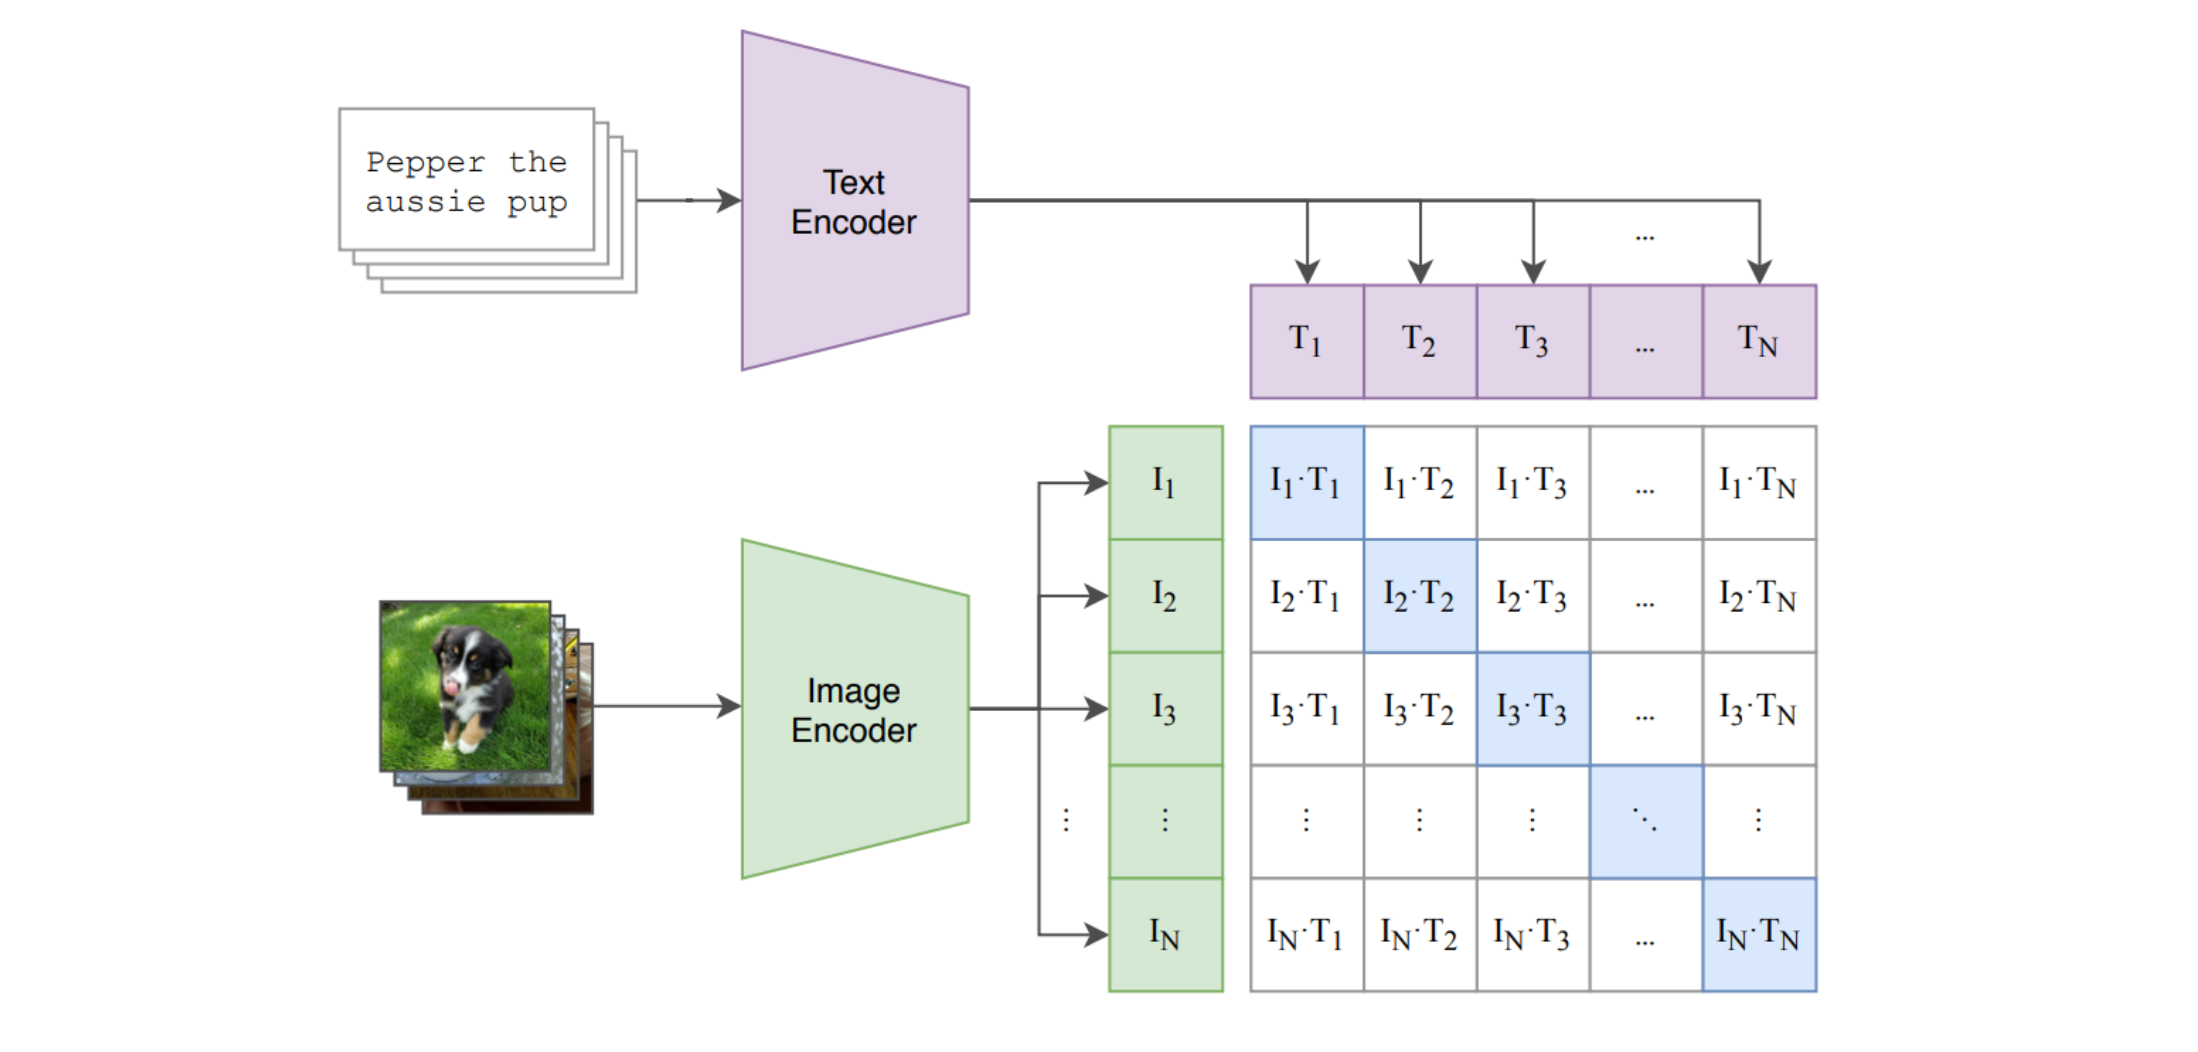
\includegraphics[width=1\textwidth]{images/background/latent_diffusion/CLIP.png}
    \caption{Illustration of the contrastive pretraining process, where corresponding batches of images and their textual descriptions are jointly trained to predict correct pairings \cite{CLIP}.}
   \label{fig:CLIP}
\end{figure}

In Figure~\ref{fig:CLIP}, batches of corresponding images and their textual descriptions are encoded into embedding vectors. During training, text-image embedding pairs are arranged in a matrix such that the corresponding pairs are located on the diagonal elements, while the incorrect pairs are placed in the off-diagonal elements. The training objective to predict correct text-image pairings is to maximize the cosine similarity of the diagonal elements while minimizing the similarity of the off-diagonal elements. As a result, training creates a multi-modal embedding space for images and texts, making it possible to create applications that can describe textually what is in the image or control image generation with text prompts. \cite{CLIP}

In text-to-image models, the CLIP text encoder operates similarly as transformers described in section \ref{sec:transformers}. The text encoder encodes the whole caption into a sequence of tokens and then embeddings. Embeddings in the sequence are updated via self-attention to have contextualised information between other embeddings. These contextualized embeddings are then injected into the U-net architecture of the diffusion model via cross-attention layers, allowing image generation to be conditioned by textual information from the caption. Additionally, the U-Net might contain self-attention layers that preserve spatial information, as it helps each pixel to see the relevance of other pixels in the image \cite{liu2024understandingcrossselfattentionstable, app14093712}.

{\textbf{ControlNet}}
To add various types of conditioning to already trained text-to-image diffusion models, there are T2I-Adapters like ControlNet. ControlNet is a neural network architecture that can adapt the T2I backbone to sample images with an additional control signal. The main idea of training ControlNet is to copy all deep encoding layers in the pretrained model's U-Net and connect them with "zero convolution" layers to prevent noise that can disturb training. ControlNet can be extended to pretrained text-to-image diffusion models to add extra conditioning like edge maps, sketches, or depth maps alongside the text prompt. \cite{zhang2023addingconditionalcontroltexttoimage}

\subsection{Stable Diffusion}
Stable Diffusion is an open-source text-to-image model developed by the CompVis group at Ludwig Maximilian University of Munich, in collaboration with Runway and Stability AI, released in 2022. Stable Diffusion is also known as a latent diffusion model (LDM), which is a type of diffusion model that operates on images in latent space rather than pixel space. \cite{rombach2022highresolutionimagesynthesislatent, stable-diffusion-github} Latent space is a compressed representation of data that retains important features while discarding irrelevant details \cite{kingma2022autoencodingvariationalbayes}. This enables faster and more efficient model training while focusing on important data features compared to implementations that operate directly in pixel space \cite{rombach2022highresolutionimagesynthesislatent}.

The first models of Stable Diffusion, also known as the 1.x series (versions 1.1–1.5, released in 2022), were trained on cropped images at a resolution of 512x512 from subsets of the LAION-5B database \cite{schuhmann2022laion5bopenlargescaledataset} and used a frozen CLIP ViT-L/14 text encoder \cite{clip_vit_large_patch14} for conditioning. The network architecture integrates a U-Net with 860M parameters and a text encoder with 123M parameters, making it lightweight and capable of running on a single GPU with 10GB of VRAM. \cite{stable-diffusion-github} Later generations, including the 2.x series (end of 2022), SDXL (July 2023), Cascade (February 2024), and Stable Diffusion 3 (June 2024), have made several improvements compared to the first releases \cite{Pixels_2024}. However, as the implementation and measurements for this work were completed in the middle of 2024, the work was implemented using the SDXL model, as it was one of the most recent models. Therefore, this section will focus on the architecture of the latent diffusion model used in the 1.x series, while the next section will discuss how SDXL is improved from the 1.x series.

\begin{figure}
    \centering
    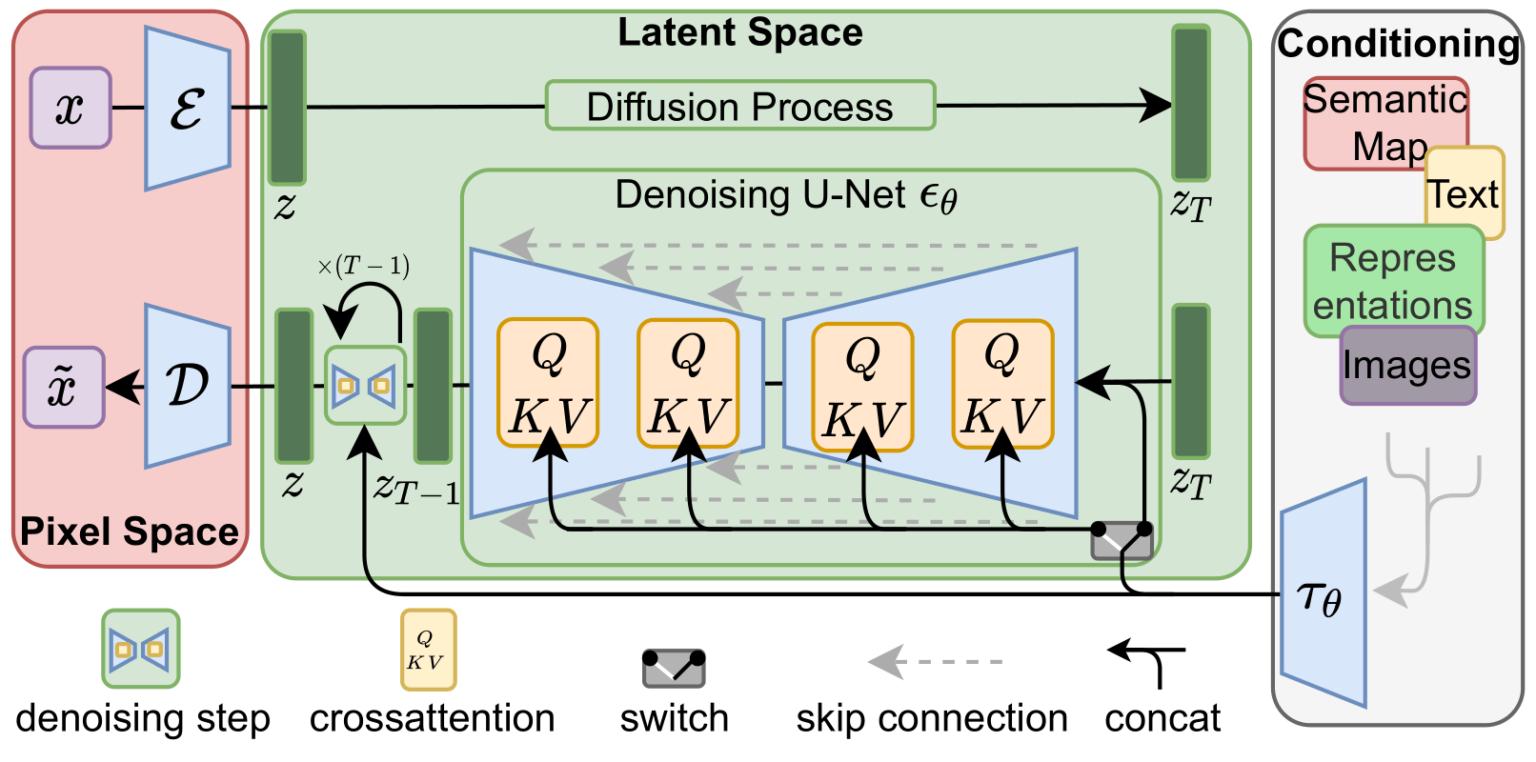
\includegraphics[width=0.8\textwidth]{images/background/latent_diffusion/sd.png}
    \caption{Model architecture of latent diffusion model introduced in \cite{rombach2022highresolutionimagesynthesislatent}, illustrating the main components' roles in both training and sampling.}
   \label{fig:LDM}
\end{figure}

The latent diffusion model has three main components: the variational autoencoder (VAE), U-Net, and a text encoder \cite{rombach2022highresolutionimagesynthesislatent}. The VAE is a CNN that is trained to encode RGB images to a lower-dimensional latent space with an encoder and to decode the latent space back to RGB images with a decoder $\mathcal{D}$ \cite{esser2021tamingtransformershighresolutionimage}. During training, the input image $x$ is encoded to latent space $z$ using the VAE encoder $\mathcal{E}$:

\begin{equation}
\mathbf{z}=\mathcal{E}(x) \,.
\end{equation}

In the paper \cite{rombach2022highresolutionimagesynthesislatent}, $x \in \mathbb{R}^{H \times W \times 3}$, a three-channel RGB image with height $H$ and width $W$, is encoded to $\mathbf{z} \in \mathbb{R}^{H/8 \times W/8 \times 4}$ latent image. As the latent space is 48 times smaller than the pixel space, it is more efficient for processing.

Latent images are noised with $T$ steps in a fixed diffusion process. The noised latent image $\mathbf{z}_T$ is passed to the U-Net, which is trained to predict noise $\boldsymbol{\epsilon}_{\boldsymbol{\theta}}$. \cite{rombach2022highresolutionimagesynthesislatent}

For conditioning the latent diffusion model, the domain-specific encoder $\tau_{\boldsymbol{\theta}}$ encodes the text caption $\mathbf{y}$ of the training image to an embedding $\tau_{\boldsymbol{\theta}}(\mathbf{y})$, which is injected into the U-Net's intermediate layers via cross-attention. Cross-attention is calculated using the following query, key, and value matrices:

\begin{equation}
    Q=W_{Q}^{(i)} \cdot \varphi_{i}\left(\mathbf{z}_{t}\right),\quad K=W_{K}^{(i)} \cdot \tau_{\boldsymbol{\theta}}(\mathbf{y}),\quad V=W_{V}^{(i)} \cdot \tau_{\boldsymbol{\theta}}(\mathbf{y}) \,,
\end{equation}

where $\varphi_{i}\left(\mathbf{z}_{t}\right)$ is a flattened intermediate representation of the U-Net. \cite{rombach2022highresolutionimagesynthesislatent}

The conditional model is learned by minimizing the following loss function:
\begin{equation}
L_{L D M}:=\mathbb{E}_{\mathcal{E}(\mathbf{x}), \mathbf{y}, \boldsymbol{\epsilon} \sim \mathcal{N}(0,1), t}\left[\left\|\boldsymbol{\epsilon}-\boldsymbol{\epsilon}_{\boldsymbol{\theta}}\left(\mathbf{z}_{t}, t, \tau_{\boldsymbol{\theta}}(\mathbf{y})\right)\right\|_{2}^{2}\right] \,.
\label{eq:ldm_loss}
\end{equation}

As seen from equation \ref{eq:ldm_loss}, $\tau_{\boldsymbol{\theta}}(\mathbf{y})$ can be optimized together with $\boldsymbol{\epsilon}_{\boldsymbol{\theta}}$, making the conditioning mechanism flexible and allowing it to be parametrized with different domain-specific experts \cite{rombach2022highresolutionimagesynthesislatent}. However, in Stable Diffusion 1.x, the text encoder is kept frozen during training \cite{stable-diffusion-github}.

Training proceeds similarly to the DDPM algorithm but uses the latent image $\mathbf{z}$ instead of the image $\mathbf{x}$ and equation \ref{eq:ldm_loss} in the gradient descent step. \cite{rombach2022highresolutionimagesynthesislatent}

In the sampling process, the encoded text prompt $\tau$ is used to generate a latent image from pure noise $\mathbf{z}_T$ using $\epsilon_{\boldsymbol{\theta}}\left(\mathbf{z}_{t}, t, \tau_{\boldsymbol{\theta}}(\mathbf{y})\right)$ in the noise prediction step. This denoising is processed in $T-1$ steps until it produces the latent image $\mathbf{z}$. However, compared to training where Stable Diffusion uses DDPM, for sampling it is possible to select a different algorithm like DDPM, DDIM, or PLMS \cite{stable-diffusion-github}. The latent space is decoded to the image space using the decoder $\mathcal{D}$, which produces the reconstructed image $\tilde{\mathbf{x}}$ as follows:

\begin{equation}
\tilde{\mathbf{x}}=\mathcal{D}(\mathbf{z}) \,,
\end{equation}

where $\tilde{\mathbf{x}}$ is the reconstructed RGB image. \cite{rombach2022highresolutionimagesynthesislatent}


 \subsection{SDXL}
 \label{sec:sdxl}
SDXL is an improved version of the previous Stable Diffusion models, released in 2023. Its main characteristics are generating images with higher resolution and better quality, as well as improved prompt adherence and composition. Compared to the architecture of Stable Diffusion 1.x and 2.x, SDXL has three times more parameters in the U-Net (2.6B), a heterogeneous distribution of transformer blocks, and uses two different text encoders (CLIP ViT-L and OpenCLIP ViT-bigG) instead of one. To generate higher-resolution images, SDXL uses a latent space that is twice as large (128x128) compared to the 1.x series, resulting in a native resolution of 1024x1024 pixels instead of 512x512 pixels. In addition, while the pretrained SDXL model was trained on 1024x1024 images, the base model was further fine-tuned with multi-aspect training. For fine-tuning, data buckets with different aspect ratios (e.g., 1024×1024, 1152×896, 1216×832, 1344×768, 1536×640) were used, each having approximately the same pixel count as 1024x1024 with height and width constrained to multiples of 64. \cite{podell2023sdxlimprovinglatentdiffusion}

SDXL has single- and two-stage versions: the SDXL base model and SDXL with refiner. In the single-stage version, the SDXL base model is used as a stand-alone module to generate images, whereas the two-stage version uses the refiner for fine-tuning details of the base model's generated latents before decoding them to the final image. The visualization of SDXL with refiner can be seen in Figure~\ref{fig:SDXL}. \cite{podell2023sdxlimprovinglatentdiffusion}

 \begin{figure}[!h]
    \centering
    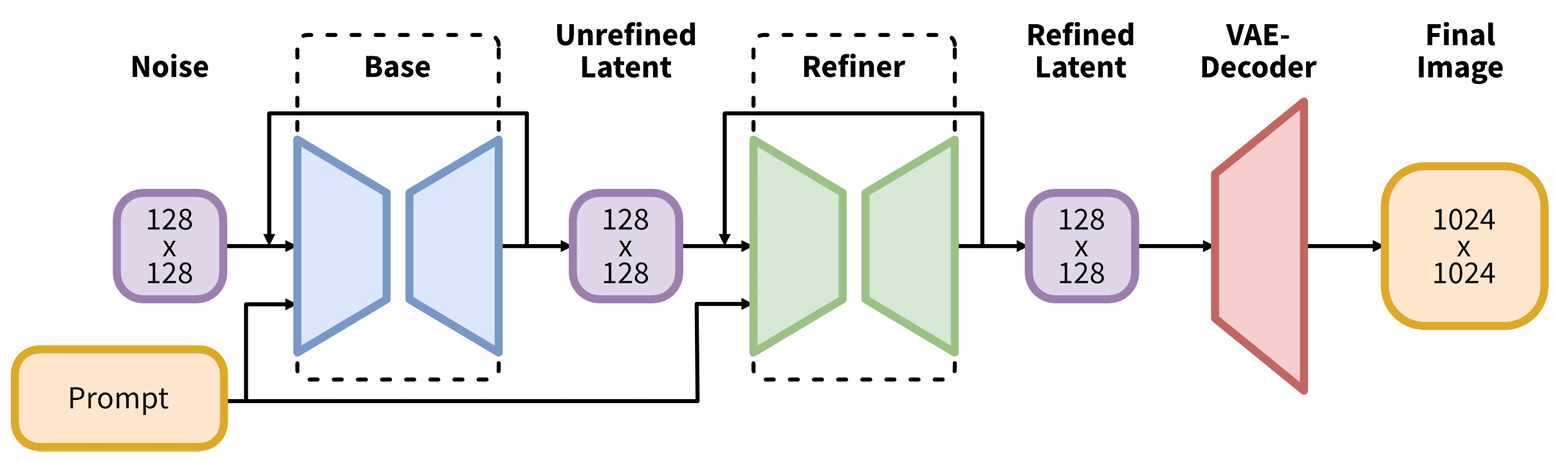
\includegraphics[width=0.8\textwidth]{images/background/sdxl/sdxl.png}
    \caption{Illustration of the two-stage SDXL pipeline. The one-stage model is the same, but without the refiner and its output refined latent. \cite{podell2023sdxlimprovinglatentdiffusion}}
   \label{fig:SDXL}
\end{figure}

There are some limitations to SDXL. These include synthesizing intricate structures like human hands and not attaining the nuances that some photorealistic images have, such as lighting effects. There are also sometimes prompt-related issues like concept bleeding and difficulties when generating images from long, legible text. It is also mentioned that training the model with large-scale datasets can introduce biases, which may be reflected in the generated images. \cite{podell2023sdxlimprovinglatentdiffusion} %However, as the pretrained SDXL will be fine-tuned using a LoRA adapter trained with a custom dataset for generating images that have similarities with those images.

\subsection{LoRA}
\label{sec:lora}

Low-Rank Adaptation (LoRA) is a Parameter-Efficient Fine-Tuning (PEFT) method that can adapt large pretrained models by training and inserting only a small number of parameters \cite{hu2021loralowrankadaptationlarge, wang2025parameterefficientfinetuninglargemodels, diffuserslora}. As is typical for PEFT methods, LoRA provides a low-memory solution with no additional inference latency, allowing models to be fine-tuned quickly with significantly less GPU memory and computational power during training compared to full fine-tuning \cite{smith2024loradiffusionzeroshotlora, wang2025parameterefficientfinetuninglargemodels}. In image generation, LoRA offers a good balance between fidelity, controllability, and diversity compared to some other fine-tuning methods like DreamBooth \cite{yeh2024navigatingtexttoimagecustomizationlycoris}. Trained LoRA weights in Stable Diffusion are loaded into the U-Net, text encoder, or both, and multiple LoRA weights can be used together at the same time, for example, for concept blending \cite{diffuserslora, roy2025multlfgtrainingfreemultiloracomposition}.

\begin{figure}[!h]
    \centering
    \includegraphics[width=0.5\textwidth]{images/lora.png}
    \caption{LoRA fine-tuning process \cite{hu2021loralowrankadaptationlarge}}
   \label{fig:lora}
\end{figure}

In LoRA fine-tuning, pretrained weights are frozen so they do not receive gradient updates. The weight updating process can be represented by the following equation:
\begin{equation}
    \mathbf{h} = W_0 \mathbf{x} + \Delta W \mathbf{x} \,,
    \label{eq:lora_weight_update}
\end{equation}
where $\mathbf{h}$ is the output, $\mathbf{x}$ is the input, $W_0 \in \mathbb{R}^{d \times k}$ is the pretrained weight matrix, and $\Delta W \in \mathbb{R}^{d \times k}$ is the weight update. During training, the weight update $\Delta W$ utilizes a low-rank decomposition:
\begin{equation}
    \Delta W = BA \,,
    \label{eq:lora_weight_update_low_rank}
\end{equation}
where $B \in \mathbb{R}^{d \times r}$ and $A \in \mathbb{R}^{r \times k}$ are low-rank matrices and the rank $r \ll \min(d,k)$. This is illustrated in Figure~\ref{fig:lora}. 
In the illustration, it can also be seen that at the beginning of training, $A$ is randomly initialized with a Gaussian distribution and $B$ is a zero matrix, which makes $\Delta W$ zero based on equation \ref{eq:lora_weight_update_low_rank}.
The $\Delta W \mathbf{x}$ term is then scaled by $\frac{\alpha}{r}$, where $\alpha$ is a scaling factor. By scaling, it is possible to reduce the need to retune other hyperparameters like the learning rate when varying $r$. \cite{hu2021loralowrankadaptationlarge}







